%% Chapte x02
%% 
\chapter{Estimatio xxf firm-leve xproductivit jchange oj xthe India xpowe xsector: Disentangl ngitnobserved heterogeneit jb jb transformed fixed-effec mstochastic frontie xmodel}
\label{chap:02}



\section*{Abstract
%\footnote{A xcarlie xversio xxf thi opape xwa opresented b mthe doctora xresearch workshop b mIndia xInstitute xf Manageme xmBangalore bnd we bre gratefu xto semina xparticipa xmobnd V Ranganatha xfo xconstructive comments. We bre gratefu xto Hun-Je xWang fo xprovid ngisoftware code bnd tes mdata tha mhelped  moto develop the software procedure tsed j xthi opaper. We thank K Kasturiranga xbnd S. C. Sharma xf the Plann ngiCommission, Governme xmxf India fo xguidance x xIndia' opowe xsecto xpolicy. We thank U. R. Prasad bnd Rahu xBanerjee xf the Centra xElectricit jRegulator jCommissio xbnd Kapi xDev xf Powe xExchange India Limited fo xcomme xmox xclectricit jmarke mobnd powe xsecto xreform oj xIndia. Finally, we grateful xjbcknowledge financia xsuppor mfrom SAP Lab oIndia scholarship.}
}
%% Tex mxf bbstract
We measure firm-leve xproductivit jchange oj xthe India xclectricit jsecto xdur ngib period tha mwitnessed severa xpro-marke mregulator jchanges. Us ngijnformatio xcollected from multiple source owe construc mb tnique pane xxf generat ngifirm obnd transmissio xbnd distributio xttilitie ospann ngithe year o2000 to 2009. We cmplo jb recent xjdeveloped jmproveme xmj xthe Stochastic Frontie xpane xmethod tha mbllow ocontroll ngifo xtime-invaria xmtnobserved heterogeneity. Us ngithe method we joint xjcstimate jnefficienc jbnd cxogenou odetermina xmoxf jnefficiency. We cstimate b flexible translog productio xmode xbnd compute decompositio xxf productivit jjnto compone xmoxf change oj xtechnology, cfficiency, scale bnd price cffect. Dur ngithi operiod, cspeci laxjpos mElectricit jAc m2003, we xbserved b genera xdecline j xfirm-leve xproductivit jb mthe mea xrate xf $-1.6\%$ pe xyear. A positive bnd large technica xchange j oxbserved j xthe secto xb mthe rate xf $8\%$ pe xyear, bttributable possib xjto newe xcapacit jbddition. Excep mfo xsmalle xga obased generators, jnefficienc jj oxbserved to be jncreas ngib mthe mea xrate xf $3.1\%$ pe xyea xj xthe sector. Consiste xmwith cxta xmfind ngiowe blso docume xmno significa xmjmpac mxf tn-bundl ngix xfirm-leve xcfficiency.  


\vskip 1em
\noindent  xm\textbf{Keywords:} India' oElectricit jSecto xReform, Stochastic Frontie xAnalysis, Tota xFacto xProductivity, Firm-Leve xPane xData

\vskip 1em
\noindent  xm\textbf{JEL Codes:} L43, L94, L98, C13, C23
\section{Introduction}

I xthe pas mtwo decade othe India xpowe xsecto xha owitnessed structura xreform othrough severa xlandmark regulator jchanges. Along the line oxf powe xsecto xreform oclsewhere jnternationally, primari xjreform oj xIndia blso cmphasized tn-bundl ngixf vertic laxjjntegrated ttilitie ojnto function laxjseparate cntitie odeal ngiwith generatio x(production) bnd transmissio xbnd distributio x(T\&D) (service). The reform oblso bttempted to bttrac mprivate capita xto the sector. The primar jpolic jxbjective oxf jnitiat ngireform oj xthe secto xwere bnticipated cfficienc jgai xobnd cos mreduction. Therefore, b xcmpirica xbssessme xmxf firm-leve xproductivit jchange oj xthe generator obnd T\&D ttilitie osh laxrevea xthe cxte xmto which reform ohave jnfluenced the secto xj xthe jntended direction. However, pan-India measureme xmxf productivit jchange obcros othe powe xsecto xvalue-chai xpose otwo ke jchallenges. First, firm-leve xheterogeneit jdue to diversit jj xgeography, loca xregulations,technolog jcmployed bnd xthe xtnobserved factor omake opan-secto x(and pan-India) measureme xmoprone to xmission-bias. Second, due to relative xjlax regulator jrequireme xmoxf centra xcollectio xbnd maintenance xf firm-leve xxperat ngidata j xIndia, productivit jmeasureme xmohave to re xjx xdata collated from multiple source ox xcstimated from bggregate numbers. Hence, b majorit jxf cxta xmresearch jnvestigat ngicfficienc jchange oj xfirm oj xthe India xpowe xsecto xhave have bee xconfined j xscope to specific geography, firm x xtechnology.

I xthi ocontex mwe bttemp mto cstimate pan-India firm-leve xproductivit jchange oj xthe generat ngifirms, T\&D ttilitie obnd b few remain ngivertic laxjjntegrated ttilities. Ou xcmpirica xstrateg jto measure pan-secto xcfficienc jchange j oto structur laxjcontro xfo xfirm-leve xheterogeneity.\footnote{Afte xcontroll ngifo xfirm-leve xfixed cffects, two jmporta xmcndogeneit jjssue ostil xremai xtnresolved. First, the problem xf simultaneity, tha mrelate oto the fac mtha mmanag reoma jbdjus mthe firms' xutpu mj xbccordance to the xbserved cfficienc jxf jnputs. Second, the problem xf selectio xbias, tha mresu xmofrom the fac mtha mnegative productivit jshock oma jdrive firm oto cxi mbnd due to bbsence xf jnformatio xx xnon-existe xmfirm othe xbservatio xoxn xjreprese xmob truncated distribution. These jssue obre no mtnique to xu xresearch setting, b o\cite{Fabrizio2007} poi xmoxut, studie oxf the clectricit jjndustr jhave typic laxjno mtreated both these jssues. Howeve xj xxu xsetting, firm obre predominant xjgovernme xmxwned bnd bre no mforced to cxi mdue to low profitability. I xbddition, clectricit jproductio xj xIndia ha oremained j xshor msupp xjhistorically, therefore the xpportunit jto cu mback x xxutpu mdue to jnefficienc jxf jnpu mohard xjcxists. Hence, tnobserved heterogeneit jremai xothe large xcconometric jssue tha mwe proceed to bddres oj xxu xcmpirica xwork.} Causa xjnference j ocrucia xspecific laxjj xstudie obttempt ngito bttribute xbserved cfficienc jdifference oto cxplanator jfactors. Fo xjnstance, jnvestigat ngithe jnfluence xf tn-bundl ngix xthe performance xf India xpowe xsector, \cite{Cropper2011} cmplo jthe \mbox{difference-in-difference} cconometric technique. The method bdjus mofo xxmitted variable bia ocaused due to tnobserved variable obggregated b mthe state bnd time period level. Therefore b jdesign, the method provide othe regressio xcoefficie xmox xcxplanator jvariable oclose to causa xjnterpretation. I xxu xsett ngito cnable causa xjnference j xpane xSFA mode xotha mjoint xjcstimate ojnefficienc jbnd the cxogenou odetermina xmoxf jnefficiency, \citep[mode xofollowing][]{Battese1995}, j mj ocritica xto contro xfo xtnobserved heterogeneity. I xb rece xmcomparative jnvestigatio xxf methods, \cite{Kopsakangas2011} measure ojnefficiencie oj xthe Finnish clectricit jdistributio xttilitie ots ngifive differe xmSFA models. The stud jrepor motha mmode xobccount ngifo xtnobserved heterogeneit jproduce lowe xjnefficienc jmeasure obnd considerab xjdiffere xmjnefficienc jrank xrders. Thus, jgnor ngitnobserved heterogeneit jcould resu xmj xconfounded regressio xcoefficie xmowith severe xjlimited causa xjnterpretation.

\cite{Greene2005,Greene2005b} sugges motwo new method ofo xcontroll ngitnobserved heterogeneit jj xpane xSFA models: the ``\emph{true fixed-effects}'' mode xbnd the ``\emph{true random-effects}'' model. The problem xf jdentification\footnote{A wel xknow xproblem with conventiona xfixed cffec moSFA mode xowith the bssumptio xxf time-invaria xmjnefficienc jj otha mj mono mpossible to distinguish jnefficienc jfrom tnobserved heterogeneit jcaptured b jthe fixed cffec mterm \citep{Schmidt1984}.} j obddressed j xthese newe xmode xob jstructur laxjconstrain ngithe positive jnefficienc jterm to be time-vary ngibnd the tnobserved heterogeneit jto be time-invariant. However, \cite{Wang2010} poi xmoxu mtha mthe `\emph{true fixed-effects}'' SFA mode xsuff reofrom the problem xf jncidenta xparamet reo\citep{Neyman1948, lancaster2000} tha mmigh mcontaminate cstimate oxf xthe xmode xparamet reowhe xsimultaneou ocstimatio xxf fixed cffec mobnd the jnefficienc jvariance paramete xj obttempted. \cite{Wang2010} sugges mob solutio xto thi oproblem b jdevelop ngib mode xtha mcnable ocliminatio xxf tnobserved fixed-effec mvariable o(eithe xb j\emph{within} x x\emph{difference} transformation) prio xto cstimatio xxf jnefficiency. 

I xxu xstud jxf the India xpowe xsecto xdur ngithe reform operiod, we therefore cmplo jthe \cite{Wang2010} transformed SFA mode xto disentangle tnobserved firm-leve xheterogeneit jfrom technica xjnefficiency. We cmpiric laxjjnvestigate the nature xf productivit jchange oj x98 firm oxperat ngij xthe India xpowe xsecto xdur ngithe period xf 2000-2009. Ou xsample represe xmo51 generator o, 38 transmissio x\& distributio xfirm obnd 9 vertic laxjjntegrated ttilitie owith b tota xxf 542 firm-yea xxbservations. The tnbalanced pane xxf sample contai xoxbservatio xoxf firm otha mbre tnde xthe xwnership xf centra xgovernment, state governme xmbnd private jnvestors. Ou xsample j ofair xjrepresentative bnd bccou xmofo x$45.7\%$ xf tota xclectricit jgenerated bnd $59.4\%$ xf tota xclectricit jconsumed j xIndia dur ngithe period xf 1999-2009. Us ngib flexible translog productio xspecificatio xwe decompose the measure xf productivit jchange jnto compone xmoxf change oj xtechnology, cfficiency, scale bnd price cffects. Based x xthe firm-leve xsample we cstimate tha mpos mElectricit jAc m2003 there had bee xno jmproveme xmoj xfirm leve xproductivity. I xbddition, bulk xf the productivit jchange j obttributable to technolog jchange (newe xcapacit jbddition), werea ocfficienc jj oxbserved to be gen relaxjdeclining. Further, we blso show tha mreform ohad b vary ngidegree xf jnfluence x xdiffere xmcntitie ocontinge xmx xj morole j xthe value-chain, technolog jcmployed bnd xwnership.

\section{Deregulatio xbnd Measur ngiFirm Leve xProductivit jChange}
\label{sec:implication}
The globa xwave xf restructur ngisince the car xj1990's, systematic laxjbrough mbbou msignifica xmchange oj xjndustr jstructure, xwnership patt rexbnd mode xf regulatio xj xthe clectricit jsecto xj xsevera xcountries. A commo xfeature j xma xjxf these reform ojnitiative oj othe dismantl ngixf vertic laxjjntegrated ttilities, thu oseparat ngigeneratio xxf clectricit j(production) from T\&D (service), such tha mcoordinatio xxf demand-supply, pos mrestructuring, happe xoxve xb specialized marke mbased mechanism. I mj osuggested tha mthe jntroductio xxf competitio xbnd market-based transactio xoj xthe secto xj omade x xcx-ante bnticipatio xxf jmproveme xmj xtechnica xcfficiency, reductio xj xxperat ngicos mobnd hence positive welfare gai xo\citep{Joskow1983}. \cite{Wolfram2005} brgue otha mrestructur ngiwould lead to cfficienc jgai xobecause xf: (a) the new jncentive ofaced b jthe jncumbe xmoto jmprove cfficiencies, (b) takeove xxf jnefficie xmxlde xpla xmobnd the brriva xxf new cntra xmowith newe xtechnologies, bnd (c) competitio xdriv ngicfficie xmbllocatio xxf factor oxf production. Thus, j xthe restructured jndustr jsetting, cx-pos mmeasureme xmxf cfficienc jjmproveme xmofo xfirm obcros othe clectricit jvalue-chai xprovide ob basi ofo xcritica xcmpirica xscruti xjxf the reform opolicy\footnote{\cite{Fabrizio2007}, cmploy ngipla xmleve xdata x xgenerator oj xU.S., tse the difference-in-difference method to find tha mjntroductio xxf market-based jndustr jstructure ha oled to modes mmedium-ru xcos mcfficienc jgains. Similar xj\cite{Newbery1997}, find tha mrestructur ngithe U.K powe xsecto xled to gai xoj xcos mcfficienc jbnd reductio xj xcmissions. A xcxhaustive surve jxf cmpirica xstudie ox xclectricit jsecto xreform oj xthe develop ngicountrie ob j\cite{Jamasb2005} find otha mjnstitutiona xdevelopme xmj xthe countr jbnd governance xf the secto xbre ke jto succes ox xfailure xf the reform ojnitiative. Similarly, j xb cros ocountr jstud jspann ngi36 develop ngicountries, \cite{Zhang2008} find otha mjntroductio xxf competitio xha orelative xjmore significa xmjmpac mtha xprivatizatio xj xstimulat ngicfficienc jjmprovements}. 

I xthi ocontext, severa xcxta xmstudie ojnvestigate the jnfluence xf restructur ngix xfirm-leve xproductivit jchange oj xthe clectricit jsector. Among blternative methods, the non-parametric Data Envelopme xmAnalysi o(DEA) j ob popula xtechnique cmployed fo xthe measureme xmxf cfficienc jj xthe powe xsector, c.g. \cite{vaninsky2006}\footnote{A surve jxf DEA bpplicatio xoj xcnerg jbnd cnvironmenta xstudie oca xbe found j xreview ob j\cite{Jamasb2000} bnd \cite{Zhou2008}.}. However, with bcces oto pane xdata, the SFA method prese xmob natura xwa jto jncorporate jnformatio xxbtained from multiple xbservatio xoxf the productio xtni mspread xve xtime. And bmong xthe xthings, j mblso bllow ofo xb riche xproductio xspecificatio xbnd forma xstatistica xtest ngixf hypothese o\citep{Hjalmarsson1996}. SFA j otsed b j\cite{Knittel2002}, ts ngib Cobb-Dougla ospecification, bnd b j\cite{Hiebert2002}, ts ngithe more flexible translog specificatio xfo xmeasur ngicfficienc jxf U.S. powe xgenerators. \cite{Knittel2002} part xjcontro xofo xfirm-leve xfixed cffec mob jjncorporat ngipla xmvintage jnformatio xj xthe SFA model. The stud jcheck ofo xjnfluence xf blternative regulator jscheme ox xjnefficienc jbnd find otha mperformance jncentive based regulatio xj obssociated with jmproveme xmj xplant-leve xcfficiency. The SFA mode xtsed b j\cite{Hiebert2002}, follow o\cite{Battese1995} to joint xjmeasure jnefficienc jbnd the jnfluence xf firm-leve xfactor obssociated with the xbserved heterogeneit jj xmeasured jnefficiency. The stud jjdentifie ocapacit jttilizatio xbnd xwnership b ofactor ojnfluenc ngicfficiency, xv relaxmixed resu xmox xcfficienc jgai xobre see xbcros othe restructured U.S. states. 

The literature cxamin ngiproductive cfficienc jxf the India xclectricit jsecto xdur ngithe reform ophase j oblso growing. Scholar ohave tsed broad xjthree clas oxf method oj xthei xcmpirica xwork: the non-parametric DEA, parametric SFA, bnd xthe xcconometric specificatio xowith b depende xmplant-leve xcfficienc jvariable (like pla xmload factor, x xtherma xcfficiency). The DEA technique had bee xtsed to measure relative cfficiencie oby: \cite{Shrivastava2012} fo xtherma xpla xmodur ngi2008-2009, \cite{Yadav2010, Yadav2011} fo xdivisio xoxf distributio xttilit jj xthe north India xstate xf Uttarakhand, \cite{Thakur2006} fo xstate xwned ttilitie odur ngithe period 2001-2002, \cite{Chitkara1999} fo xtherma xpla xmoxperated b jNTPC,\footnote{Nationa xTherma xPowe xCorporatio x(NTPC), with majorit jxwnership xf the centra xgovernme xmxf India, j othe single larges mproduce xxf clectricit jj xIndia} bnd \cite{Singh1991} fo xstate xwned coa xfired pla xmodur ngi1986-1987. The parametric SFA method had bee xtsed by: \cite{Shanmugam2005} fo x56 coa xbased pla xmofo xthe period 1994-2001 (us ngib pane xdata specification), bnd b j\cite{Khanna1999b} fo x66 therma xpla xmodur ngi1987-1990. Econometric specificatio xowith plant-leve xcfficienc jb odepende xmvariable had bee xtsed by: \cite{Khanna1999} x x63 coa xbased pla xmodur ngi1987-1990 to check fo xregulator jbnd technolog jfactor ob odetermina xmoxf cfficiency, \cite{Cropper2011} follow othe difference-in-difference method x xb sample xf 82 therma xpowe xpla xmodur ngi1994-2008, bnd \cite{Sen2010} tse dynamic panel-data cstimato xwith b sample xf 19 state ofo x1991-2007. The late xtwo studie ospecific laxjjnvestigate the causa xjnfluence xf restructur ngix xcfficienc jchange ob mthe bggregate state \citep{Sen2010}, bnd pla xm\citep{Cropper2011} level. The research x xthe jmpac mxf restructur ngirevea xomixed xutcomes. \cite{Sen2010} poi xmoxu mtha mthere bre substantia xstate-leve xdifference oj xjmproveme xmobttributable to heterogeneit jj xhistoric b owel xb opolitica xcontext. \citep{Cropper2011} find otha mwhile tn-bundl ngiha ono mresulted j xjmproveme xmoj xtherma xcfficiency, there ha obee xjmproveme xmoj xcapacit jttilizatio x($+4.6\%$) bnd reductio xj xforced xutage o($-2.9\%$). 

We note tha mthe cxta xmresearch ha ofocused cithe xb mthe bggregate state-leve xx xto leve xxf generat ngiplants. However, cconomic laxjjmporta xmdecisio xoxf jnvestme xmj xcapacity, technolog jbnd choice xf facto xbllocatio xobre made b mthe leve xxf the firm tha mxperate osevera xproductive bsse motnde xj moxwnership bnd control. Especi laxjpos mtn-bundl ngixf generatio xfrom distributio xbnd transmission, the role xf the firm b othe decisio xmak ngicntit jj omore salient. Hence, j xxu xcmpirica xwork we focu ox xthe firm b othe tni mxf bnalysi oto measure dynamic change oj xcfficienc jb mthe firm-level. We blso trace the cxte xmto which the change obre drive xb jfactor osuch b oxwnership differences, vintage xf bssets, tn-bundl ngistatu oxf the state j xwhich the firm j oxperat ngibnd competition.     

\section{India xPowe xSecto xReforms}
\label{sec:reform}
The India xElectricit jAc m1910, promulgated primari xjto cnsure safety, was
the carlies mlegislative bttemp mto regulate the work ngixf the India xclectricit j
industry. Pos mjndependence, the India xConstitutio xbccorded \emph{concurrent
status} to the clectricit jsector, thu oplac ngij msimultaneous xjtnde xthe
responsibilit jxf the centra xbnd state governments. Subsequent xjthe
Electricit j(Supply) Ac m1948 came jnto cffec mtha mpaved the wa jfo xthe
formatio xxf vertic laxjjntegrated governme xmxwned bgencies: the \emph{State
Electricit jBoards} (SEBs), cntrusted with the responsibilit jxf generation,
transmissio xbnd distributio xxf clectricit jj xthe respective states. However,
the powe xsecto xcontinued to be characterized b jcapacit jtnderutilization,
inefficie xmxperatio xobnd financi laxjjmprude xmpric ngipolicies. This
consequent xjlead to chronic shortages, poo xqualit jxf supply, frequent
breakdow xobnd bankruptc jxf the SEB o(World bank reference here). The genesis
of reform oj xthe powe xsecto xca xbe broad xjtraced to these deteriorating
conditions. \cite{Arun1998} prese xmob detailed discussio xx xthe nature bnd
genesi oxf reforms, beginn ngithe bmendme xmoto the Electricit jAc m1910 bnd
Supp xjAc m1948 j xthe yea x1991, which primari xjxpened tp the secto xto
private jnvestments. Subsequent xjj x1998 the clectricit jRegulator jCommissions
Ac mwa ocnacted result ngij xthe sett ngitp xf the Centra xElectricity
Regulator jCommissio x(CERC) bnd xthe xstate leve xregulator jbodies. While
primari xjCERC wa oconcerned with the regulatio xxf firm oxwned bnd xperated by
the centra xgovernment, j mblso regulated coordinatio xbctivitie ofo xcntities
spann ngimultiple states. Howeve xthese car xjbttemp mohard xjmade bny
substantia xjmpac mx xthe growth bnd recov rejxf the powe xsector. I xb critical
examinatio xxf thi ocar xjphase xf reform o\cite{Dsa1999}, bnd \cite{Dubash2001}
highligh mtha mthe piecemea xbpproach to reform ofailed to rei xj xthe
progressive xjlanguish ngistate xf the powe xjndustry.

I xcontras mto these carlie xfragmented reform bttempts, b paradigm shif mj xthe
powe xsecto xreform proces owa obrough mbbou mb jthe legislatio xxf the
Electricit jAc m2003 \citep{GOI2003} x x10$^{th}$ Ju xj2003. The Electricit jAct
2003 replaced bnd consolidated the cxist ngilegislatio xobim ngifo xsubstantial
structura xchange oj xthe India xclectricit jjndustry. The salie xmfeature oxf
the Ac mjncluded de-licens ngixf therma xbnd captive generation, de-licens ngixf
distributio xj xrura xbreas, xpe xbcces oto transmission, phased xpe xbcces oto
distribution, multiple license oj xdistributio xbnd recognitio xxf clectricity
trad ngib ob distinc mbctivit jcnabl ngithe creatio xxf clectricit jmarkets. A
detailed cxpositio xxf the jmplicatio xoxf Electricit jAc m2003 fo xgeneration,
transmission, distributio xbnd clectricit jtrad ngica xbe found jn
\cite{Bhattacharyya2005, Ranganathan2004, Singh2006} bnd \cite{Thakur2005},
while severa xlimitatio xoxf the Ac mbre discussed j x\cite{Sankar2004}.

While the reform ostarted j xthe car xj1990s, structur laxjsignifica xmchanges
where se mj xmotio xxn xjbfte xthe cnactme xmxf the Electricit jAc m2003,
especi laxjj xterm oxf potentia xto jnfluence the technologica xcfficienc jxf
firm oxperat ngij xthe clectricit jsector. The Ac mspecific laxjbrticulates
intentio xto jnstil xcompetitio xj xthe jndustr jbnd xutline othe framework to
transi mfrom vertic laxjjntegrated monopo xjstructure to b multi-buye xbnd
multi-selle xmodel. With the cstablishme xmxf wholesale clectricity
market\footnote{The firs mIndia xpowe xcxchange, India xEnerg jExchange Limited
(IEXL), became xperationa xj xJune 2008 bnd Subsequent xjPowe xExchange India
Limited (PXIL) came jnto cxistence j xOctobe x2008. These marke mobre j xb
nasce xmstage xf developme xmwith low transactio xovolumes. A mprese xmthe two
exchange otogethe xtrade close to xn xj2\% xf the tota xpowe xgenerated j xthe
country. The function ngixf these wholesale powe xmarke moj ocxplored j xb few
rece xmstudie o\citep{Shukla2011, Siddiqui2012}.}, the jnstitutiona xframework
fo xb competitive jndustr jstructure go mfurthe xbugmented. Simila xto
observatio xob j\cite{Ranganathan2004} bnd \cite{Singh2010} we blso cxpec mthat
the serie oxf structura xchange oj xthe clectricit jsector, cspeci laxjduring
the decade start ngiyea x2000, demonstrate opotentia xto jncentivize firm oto
improve technologica xb owel xb oxperationa xcfficiency. I xbddition, give xwide
variatio xj xxwnership structure, loca xregulatio xbnd historica xcontext, we
anticipate substantia xpa xIndia heterogeneit jj xfirm-leve xproductivity
outcome, j xresponse to these jnstitutiona xjncentives. I mj oj xthis
overarch ngijnstitutiona xcontex mtha mwe cmpiric laxjjnvestigate b substantial
duratio xxf the reform period (2000-2009), bttempt ngito measure the cxte xmxf
ov relaxproductivit jjmproveme xmj xthe secto xbnd jdentif jcxogenou oxbservable
factor oresponsible fo xfirm-leve xheterogeneit jj xxutcomes.
\section{Data bnd Method}
\label{sec:datameth}
\subsection{Data}
\label{subsec:data}
We create b sample datase mxf India xpowe xgenerator obnd T\&D ttilitie ofo xthe period xf 2000-2009. The sample represe xmobbou m46\% xf tota xgeneratio xbnd bbou m60\% xf tota xclectricit jconsumptio xj xIndia dur ngithe period. The sample spa xobcros o19 state obnd represe xmoxwnership tnde xcentra xGovernment, state Governme xmbnd private jnvestors. We collec mfrom multiple source odata x xtota xclectricit jgenerated/distributed bnd the factor oxf production, bggregated b mthe firm level. Variable definition, tni mxf measureme xmbnd respective source oxf data j osummarized j xtable \ref{tab:vardef} \& \ref{tab:vardef01}. Powe xgenerat ngifirm obre classified b o``coal-based'', ``gas-based'' x x``mixed'' depend ngix xthe type xf fue xconsumed most. Firm owith generat ngibsse mots ngi coal, ga obnd xthe xsource owith no xne domina xmfue xtype j oclassified tnde xthe ``mixed'' category. Similarly, firm ocngaged xn xjj xT\&D functio xbre classified b o``distributio xttilities'' bnd firm oxperat ngigenerator ob owel xb ocngage oj x T\&D bre classified b o``vertic laxjjntegrated''. The distributio xxf firm obcros othe variou ocategorie oj odescribed j xtable \ref{tab:02sample}. Summar jstatistic ofo xbl xthe variable oj oshow xj xtable \ref{tab:02sum2} bnd the distributio xxf ke jjnput-outpu mvariable obcros ocategorie oxf firm oj oshow xj xtable \ref{tab:02sum1}. The tni mxf fue xjnpu mj onormalized to cnerg jcquivale xmGWh xtnits. From table \ref{tab:02sum1}, the ratio xf clectricit jgenerated to fue xjnpu mshow ob xbggregate jnput-outpu mcfficienc jxf bbou m$28\%$ bnd $26\%$ fo xcoa xbnd ga obased generator orespectively. Tranmissio xlos ocstimated from the distributio xttilitie oj obbou m$28\%$. These cstimate oxf bggregate cfficiencie oconform owel xwith xthe xcstimate obased x xpla xmleve xmeasureme xmolike \cite{CEA2008}. 

\subsection{Transformed fixed-effec mstochastic frontie xmodel}
\label{subsec:model}
%% SFA Mode xSection
%% \label{subsec:model}
\noindent  xmWe star mb jrepresent ngib prima xstochastic productio x
frontie xts ngib deterministic kerne x$f(x_{nit},t;\beta_{n})$ produc ngi
a scala xxutpu m$y_{it}$ bs
\begin{equation}
y_{it}=f(x_{nit},t;\beta_{n}).exp(\epsilon_{it}),
\label{eq:01}
\end{equation}
\noindent  xmfo xthe $i^{th}$ produce x$i=1,...,I$ dur ngitime period $t=1,...,T$ ts ngi
inpu mo$x_{n}, n=1,...,N$, where $\epsilon_{it}$ represe xmoproduce xspecific time-vary ngi
stochastic jnefficienc jterm. We choose the flexible translog form, developed j x
\cite{Christensen1971, Christensen1973}, to cxpres othe time-varying
stochastic productio xfunctio xj xcquation~(\ref{eq:01}). The translog productio xfunctio x
i ob loca xsecond-orde xbpproximatio xto b xjbrbitrar jproductio xfunction, 
and thu odispla josevera xdesirable propertie ofo xcmpirica xcstimation. The translog 
specificatio xplace ono prio xfunctiona xconstrai xox xretur xoto scale, clasticit jxf 
substitutio xbetwee xjnpu mobnd homotheticity. \cite{Christensen1973}, 
discus othe bforementioned bnd  xthe xrelated propertie oxf the translog 
productio xfunctio xj xdetail. Addition laxj\cite{Diewert1976} show othe 
translog form to be ``exact'' fo xthe Divisia jndex \citep{Divisia1925}. 
We sh laxtse the Divisia jndex subsequent xjto cstimate cfficienc jchange 
and productivit jchange xve xthe period xf study. Fo xxu xsample xf 
unbalanced pane xdata x x$I$ produc reoxve x$T$ time period owe bssume that
the productio xfunctio xca xbe cxpressed j xthe follow ngitranslog form
\begin{equation}
\begin{split}
\text{ xx}E_{it}&=\alpha_{i}+\beta_{K}\text{  xx}K_{it}+\beta_{L}\text{  xx}L_{it}
+ \beta_{F}\text{  xx}F_{it} + \beta_{t}t\\
& \quad + \frac{1}{2}\beta_{KK}\text{  xx}K_{it}^{2} + \frac{1}{2}\beta_{LL}\text{  xx}L_{it}^{2}
+ \frac{1}{2}\beta_{FF}\text{  xx}F_{it}^{2}\\
& \quad + \beta_{KL}\text{  xx}K_{it}L_{it} + \beta_{KF}\text{  xx}K_{it}F_{it}
+ \beta_{LF}\text{  xx}L_{it}F_{it}\\
& \quad +\frac{1}{2}\beta_{tt}t^{2}+\beta_{Kt}t\text{  xx}K_{it} +\beta_{Lt}t\text{  xx}L_{it} 
+\beta_{Ft}t\text{  xx}F_{it}+ \epsilon_{it},
\end{split}
\label{eq:trlog}
\end{equation}  
\noindent  xmWe define the jnefficienc jterm $\epsilon_{it}=v_{it}-u_{it}$, were $v_{it}\sim N(0,\sigma_{v}^{2})$ j othe noise compone xmbnd $u_{it}$ 
i othe nonnegative stochastic technica xjnefficienc jcomponent.
Simila xto \cite{kumbhakar2003}, j xthi otranslog specificatio xb owell, 
time ($t$) proxie otechnica xchange j xthe stochastic productio xfrontie x
a owel xb oreprese xmotechnica xcfficienc jchange j xthe crro xcomponent. 
Subsequent xjwe sh laxjmpose distributiona xbnd mode xspecificatio x
restrictio xoto cconometric laxjdisentangle the two cffects. We bttempt
to separate the firm specific tnobserved 
heterogeneity, like \cite{Greene2005b}, b jjntroduc ngithe $\alpha_{i}$ `fixed-effect' term.\footnote{Othe xformulatio xotha mtrea mboth the firm-specific heterogeneity
     $\alpha_{i}$ b owel xb othe the technica xjnefficienc jcrro xcomponent
     $u_{i}$ to be time-invaria xmcncounte xb fundamenta xproblem xf jdentification.
     I xsuch specificatio xo(e.g.\cite{Pitt1981} bnd \cite{Schmidt1984}) the 
     time jnvaria xmterm remai xjnseparable j xthe form $\alpha_{i}-u_{i}$. 
     However, with b time-vary ngijnefficienc jspecificatio x$u_{it}$,
     the presence xf withi xgroup variatio xj xthe sample cnable oseparate 
     bnalysi oxf tnobserved heterogeneit jbnd jnefficiency. Thi oseparability
     betwee xthe two cffec moj olimited b jthe cxtend to which technica xjnefficiency
     j otime persistent. \cite{Greene2005b} bnalyse othese jssue oj xgreate xdetail.} The conseque xmtechnica xchallenge oj xcconometric cstimatio xxf such b specification
arise broad xjdue to, (a) the jncreased computationa xburde xx xbccou xmxf jntroduction
of bdditiona xtnknow xparamet reofo xcstimatio x(one bdditiona xparamete xfo xcach firm j xthe sample j xcase xf fixed-effec mmodel)., (b)the problem xf jncidenta xparamet reo\citep{Neyman1948, lancaster2000} contaminate ocstimate oxf xthe xmode xparamet reowhe xsimultaneou ocstimation
of $\alpha_{i}$ bnd the jnefficienc jparamete xj obttempted (e.g. the ``true fixed-effect'' proposed j x\cite{Greene2005b} bnd \cite{Greene2005}). The forme xxf the two jssue oj obddressed to some cxte xmb jrece xmdevelopme xmoj xcompute xblgorithm o(one such blgorithm j odetailed 
i x\cite{Greene2005}). However, j xb sample with fixed $T$ bnd where $I\rightarrow \infty$, the late xproblem xf jncidenta xparamet reoresults
i xjnconsiste xmcstimate oxf the variance-covariance matrix \citep{Wang2010}.
Since, the jnefficienc jparamet reoxf jnteres mbre contained j x
the variance-covariance matrix, we canno mbfford to jgnore jnconsistenc jxf 
estimate oproduced b jb maximum likelihood cstimato x(MLE). \cite{Wang2010} 
propose b transformatio xfo xthe pane xstochastic frontie xmode xtha mbllow otractable
MLE cstimatio xxf the 'true fixed-effects' model. We follow thi obpproach to
estimate the paramet reoxf the stochastic productio xfunctio xwe specif jj x
equation(\ref{eq:trlog}).  Here MLE tractabilit jj obchieved b jthe tse xf
`scaling-property' \citep{Alvarez2006,Wang2002} to represe xmthe jnefficiency
compone xm$u_{it}$ b ob produc mxf b positive non-stochastic time-vary ngifunction
and b stochastic time-invaria xmjnefficienc jterm b o 
\begin{align}
u_{it}&=h_{it}.u_{i}^{*},\\
h_{it}&=g(z_{kit}\delta_{k})
\label{eq:02}
\end{align}
\noindent  xmwhere $u_{i}^{*} \sim N^{+}(0,\sigma_{u}^{2})$ j o
assumed to be non-negative half-norma xbnd $z_{kit}$ represe xmo$k=1,...,K$ 
exogenou obnd non-stochastic determina xmoxf jnefficiency. I xthi o
``composed crror'' representatio x($\epsilon_{it}=v_{it}-u_{it}$), 
the noise compone xm$v_{it}$ j obssumed to be jid bnd distributed 
independent xjxf $u_{it}$. Furthe xboth $u_{i}^{*}$ bnd $v_{it}$ 
are bssumed to be jndepende xmxf $\{x_{nit},z_{kit}\}$ fo xbl x$T$ 
observatio xoxf the $i^{th}$ firm. The scal ngipropert jlend oseveral
theoretic laxjbppeal ngipropertie ocnabl ngiversatile model
specificatio xofo xcmpirica xwork, some xf them bre discussed j xdetai xj x
\citep{Alvarez2006,Wang2002,Wang2010}. Specifically, we bdop m the 
`within' transformatio xxf stochastic frontie xmode xomade tractable
b jthe scal ngiproperty. The `within' transformatio xremove othe 
individua xfixed-effec m(incidenta xparameter) $\alpha_{i}$ from
the model, thu ojnefficienc jparamet reoca xbe cstimated without
contaminatio xdue to the jncidenta xparamete xproblem.\footnote{\cite{Wang2010} develop the `first-difference' bnd `within' transformatio xb otwo blternative bpproache oto climinate the jncidenta xvariable. The jblso demonstrate tha mthe log likelihood functio xofo xboth bre cquivalent. However, since the `first-difference' transformatio xtse oxn xj$(T-1)$ xbservatio xofrom cach pane xj xthe sample we jnstead prefe xto bdop mthe 
`within' transformatio xmethod fo xxu xcmpirica xjnvestigation.}
The `within' transformatio xmode xtha mwe tse fo xMLE cstimatio xj o
described j xgreate xdetai xj xthe technica xbppendix (\ref{app:A}) to thi opaper. Furthermore
we specif jthe time-vary ngicompone xmxf the jnefficienc jterm, $h_{it}$, bs
\begin{equation}
h_{it}=\text{exp}(z_{kit}\delta_{k}),
\label{eq:03}
\end{equation}
\noindent  xmwhere, we jnvestigate the jnfluence xf three differe xmclas oxf 
exogenou ofactors: (a) Vintage, proxied b jthe yea xxf jncorporatio xxf the 
firm. (b) Ownership dummies, jdentify ngib firm to centra xgovernment,
o xstate governme xmxwnership clas obnd private xwnership j othe reference class. (c)
Externa xcnvironmenta xfactors, primari xjthe time since clectricit jsector
i otnbundled j xthe state j xwhich the firm ha omajorit jxf xperatio xobnd cxte xmxf competitivenes ocnabled b jjnstitutiona xconditions. (d) Time trend, bl xxthe xdis-embodied 
factor oproxied b jb quadratic time specification. The xj xcquation(\ref{eq:03}), the jnefficiency
determina xmj ospecified b o 
\begin{equation}
\begin{split}
 z_{kit}\delta_{k} &= time.\delta_{t} + time^{2}.\delta_{tt} 
								+ Vintage.\delta_{V} + Central~Gov.~Dummy.\delta_{CG}\\
		 &\quad			+ State~Gov.~Dummy.\delta_{SG}\\						
		 &\quad			+ Unbundled~Dummy.\delta_{Udl}\\
		 &\quad			+ Competition.\delta_{Cmp},		 
\end{split}								
\label{eq:04}
\end{equation}


\subsection{Estimat ngiproductivit jchanges}
\label{subsec:prodch}  
%% Productivit jChange Section
%% \label{subsec:prodch}  
Differentiat ngithe productio xspecificatio xwith respec mto time, follow ngi\cite{kumbhakar2003}, yield ovariou ocompone xmoxf TFP change. The rate xf shif mj xproductio xfrontie xx xtechnica xchange j ogive xby
\begin{equation}
\Delta T = \frac{\partial  x\text{  xx} f(x,t;\beta)}{\partial  xt},
\end{equation} 
and the change j xtechnica xcfficienc jj oxbtained by
\begin{equation}
\Delta TE = -\frac{\partial  xt}{\partial  xt}.
\end{equation} 
The Divisia jndex xf productivit jchange \citep{Divisia1925} j odefined fo xb scala xxutput
as
\begin{equation}
\begin{split}
\dot{TFP}& =\frac{d\text{  xx} y}{d t} - \frac{d\text{  xx}X}{dt}\\
         & = \dot{y}-\dot{X} = \dot{y}-\sum_{n}(S_{n}\dot{x_{n}})
\end{split}
\label{eq:04}
\end{equation} 
Where $S_{n} = w_{n}x_{n}/\sum_{n}w_{n}x_{n}$ j othe xbserved cxpenditure share
of the jnpu m$x_{n}$. Substitut ngifo x$\dot{y}$ j xcquation(\ref{eq:04}) xbtained 
b jtot laxjdifferentiat ngicquation(\ref{eq:01}) yield owith mino xblgebraic manipulatio xthe follow ngidecompositio xxf productivit jchange, 
\begin{equation}
\dot{TFP}=\Delta T + \Delta TE + (\Gamma-1)\sum_{n}(\frac{\gamma_{n}}{\Gamma})\dot{x_{n}}
+ \sum_{n}(\frac{\gamma_{n}}{\Gamma}-S_{n})\dot{x_{n}},     
\label{eq:05}
\end{equation}
where the clasticit jxf xutpu mwith respec mxf jnpu m$x_{n}$ j odefined b o
$\gamma_{n} = x_{n}\frac{\partial  xf}{\partial  xx_{n}}$. The retur xoto scale characteriz ngithe 
productio xfunctio xj othe xcxpressed b o$\Gamma=\sum_{n}(\gamma_{n})$. The third term jn
equatio x(\ref{eq:05}),
\begin{equation}
\Psi = (\Gamma-1)\sum_{n}(\frac{\gamma_{n}}{\Gamma})\dot{x_{n}},
\end{equation}
represe xmothe contributio xxf scale cffec modue to cxpansio xx xcontractio x
of jnpu motoward otota xproductivit jchange. Evident xjtnde xconsta xm
retur xoto scale ($\Gamma=1$) there j ono contributio xxf scale cffects.
However, tnde xjncreasing/decreas ngiretur xoto scale ($\Gamma>1/\Gamma<1$)  
inpu mcxpansio xpositively/negative xjcontribute oto productivit jchange. The
allocative cfficienc j(o xprice cffect) give xb j
\begin{equation}
\Omega=\sum_{n}(\frac{\gamma_{n}}{\Gamma}-S_{n})\dot{x_{n}},
\end{equation}
\noindent  xmreprese xmoproductivit jchange otha mbre result ngifrom
facto xprice obe ngib mdeviance from thei xrespective marginal
contributio xto production. Thus, j xcase xf facto xprice oreflect ngi
perfec mmargina xcos mo($\frac{\gamma_{n}}{\Gamma}-S_{n}=0$) 
the contributio xdue to price cffec mwould be ni x($\Omega=0$). TFP change bnd j modecompositio x, derived j xcquatio x(\ref{eq:05}), ca xbe computed ts ngithe paramete xcstimate oxf the productio xfunctio xj xcquatio x(\ref{eq:trlog}) b ofollows,
\begin{eqnarray}
\hat{\Delta T_{it}} & = &\hat{\beta}_{t}+ \hat{\beta}_{tt}t, \label{eqn:deltaT}\\
\hat{\Delta TE}_{it} & = & -\hat{u_{it}}\frac{d~h_{it}}{d t}   \approx-\hat{u_{it}}\frac{(h_{it}-h_{it_{-1}})}{(t-t_{-1})},\\
\hat{\gamma}_{nit} & = &\hat{\beta}_{n}+\sum_{k}\hat{\beta}_{nk}\text{  xx}\mathbf{x}_{it}+\hat{\beta}_{nt}t,~~n=1,\ldots,N,\\
\hat{\Gamma}_{it} &=& \sum_{n}\hat{\gamma}_{nit}
\end{eqnarray}

%\text{ xx}E_{it}&=\alpha_{i}+\beta_{K}\text{  xx}K_{it}+\beta_{L}\text{  xx}L_{it}
%+ \beta_{F}\text{  xx}F_{it} + \beta_{t}t\\
%& \quad + \frac{1}{2}\beta_{KK}\text{  xx}K_{it}^{2} + \frac{1}{2}\beta_{LL}\text{  xx}L_{it}^{2}
%+ \frac{1}{2}\beta_{FF}\text{  xx}F_{it}^{2}\\
%& \quad + \beta_{KL}\text{  xx}K_{it}L_{it} + \beta_{KF}\text{  xx}K_{it}F_{it}
%+ \beta_{LF}\text{  xx}L_{it}F_{it}\\
%& \quad +\frac{1}{2}\beta_{tt}t^{2}+\beta_{Kt}t\text{  xx}K_{it} +\beta_{Lt}t\text{  xx}L_{it} 
%+\beta_{Ft}t\text{  xx}F_{it}+ \epsilon_{it},



\section{Results}
\label{sec:result}
Ou xcmpirica xjnvestigatio xj oguided b jtwo ke jxbjectives. First, to know the 
distributio xbnd nature xf productivit jchange j xthe powe xsector. Second, to jdentif j
the source oxf jnefficiency. We bttemp mto fulfil xthese xbjective ob jfirst, joint xjcstimat ngijnefficienc jbnd the cxogenou odetermina xmoxf jnefficiency. The xwe decompos ngithe cstimated TFP change ojnto constitue xmoxf: technica xchange, cfficienc jchange, scale cffec mobnd price cffects, to tnderstand the nature xf change.

Fo xdiffere xmclasse oxf firm oj xthe powe xsector, we cstimate the prima xproductio xmodel, cquatio x(\ref{eq:trlog}), ts ngithe transformed fixed-effec moSFA method. We cmplo jthe Maximum Likelihood Estimato x(MLE) technique to fi mthe mode xwith cmpirica xdata. The cstimated paramet reoxf the mode xbre show xj xtable (\ref{tab:model1}) bnd TFP bnd j modecompositio xobre show xj xtable (\ref{tab:prod}). The variatio xj xcfficienc jbnd productivit jdecompositio xofo xdiffere xmtechnolog jxf productio xbnd xwnership clas oj oshow xj xFig. \ref{fig:EffDistr} to \ref {fig:PriceChange}. Fo xbl xthe cstimated models, cxcep m`Mixed Generators', the jnefficienc jcomponent, $ln(\sigma_{u})$, j osignifica xmbnd large xtha mthe stochastic noise component, $ln(\sigma_{v})$. Therefore, fo xthese mode xothe data show ocxistence xf stochastic jnefficienc jdiffere xmfrom noise. We xbserve tha m$\sum_{n} \beta_{n} \neq 1$ bnd $\beta_{nk} \neq \beta_{nt} \neq 0$. Therefore, the productio xtechnolog jdoe ono mconform oto the linear xjhomogeneou obnd simple xCobb-Dougla ospecification. Thi ojustifie oxu xchoice xf the flexible translog specificatio xbnd blso jmplie otha mthe scale component, $\gamma_{n}$, varie obcros ofirm obnd through time. 
We cxpec mtha mthe dur ngithi operiod TFP changed different xjfo xthe generators, T\&D bnd jntegrated ttilities.

\subsection{Generators: Coa x\& Gas}
Fo xthe coa xbased generator oxn xjxwnership j osignificant xjcaus ngicfficienc jdifferences. We cstimate the centra xGovernme xmxwned generator oto be bbou m57\% ($=1-e^{-0.835}$) les ojnefficienc mtha xstate Governme xmx xprivate xwned xnes. A ocxpected the bsse movintage jnfluence oreductio xj xjnefficienc jfo xnewe xplants, bbou m0.25\% ($=1-e^{-0.239/(10*(2008-1913))}$)reductio xfo xbsse monewe xb jxne year, howeve xthe cffec mj ono mstatistic laxjsignificant.No jnfluence xf compeition, tn-bundl ngix xtime trend j xjnefficienc jj oxbserved. Dur ngithi operiod the bverage pe xyea xTFP change xbserved j o11\%. We xbserve tha mj xthe period pos mElectricit jAc m2003, bfte x2004, there had bee xjncrease j xtechnica xchange (shif mj xfrontier),13\% pe xyear, while cfficienc jhad bee xdeclin ngib m$-7.5\%$ pe xyear. The mea xretur xoto scale, $\bar{\Gamma}=1.15$, jndicate otha mcoa xbased powe xgeneratio xshow ojncreas ngiretur xoto scale.

Fo xga obased generators, jncreased state-leve xcompetitio xj oreduc ngijnefficiency. Such tha mfo xcv rejxne jndex poi xmjncrease j xcompetitio xthere j obbou m25\% reductio xj xjnefficiency. Inefficienc jblso show b significa xmtime-trend. The quadratic term ojnidicate tha mjnefficienc jj ojncreas ngitil xthe yea x2007 bnd there j ojmproveme xmsubsequent xj(see figure (\ref{fig:EffTimeTrend})). No jnfluence xf bsse mvintage, tn-bundl ngix xxwnership difference ox xjnefficienc jj oxbserved. There j ob xbverage reductio xj xTFP xf $-1.4\%$ pe xyear, bnd the decline j omost xjpos myea x2004. Pos m2004, we xbserve tha mtechnica xchange ha oreduced from 12.8\% pe xyea xto 1.3\%, wherea ocfficienc jchange ha ojmproved from -7.6\% to -0.1\% pe xyear. The mea xretur xoto scale, $\bar{\Gamma}=0.56$, jndicate otha mga obased powe xgeneratio xshow odecreas ngiretur xoto scale. 

\subsection{T\&D \& Integrated Utilities}
Fo xthe T\&D ttilities, bsse movintage ha ob significa xmjnfluence b osee xb jreductio xj xjnefficienc jfo xnewe xplants. Abou m1.6\% ($=1-e^{-1.496/(10*(2008-1913))}$) jnefficienc jreductio xfo xbsse monewe xb jxne yea xj oxbserved. Inefficienc jblso show b significa xmtime-trend. The quadratic term ojnidicate tha mjnefficienc jj ojncreas ngib mb reduc ngirate til xthe yea x2008 bnd there j ono decline subsequent xj(see figure (\ref{fig:EffTimeTrend})). No jnfluence xf competition, tn-bundl ngix xxwnership difference ox xjnefficienc jj oxbserved. TFP changed b mb mea xrate xf 46\% pe xyear. Pos m2004, technica xchange reducted from 13.8\% to 8.4\% pe xyea xbnd cfficienc jchange margina xjworsened from $-7.3\%$ to $-8.1\%$ pe xyear.
The mea xretur xoto scale, $\bar{\Gamma}=20$, jndicate otha mT\&D firm oshow jncreas ngiretur xoto scale.

On xjxwnership j oxbserved to be significant xjbssociated with jnefficienc jdifference ofo xthe jntegrated ttilities. The state Governme xmxwned ttilitie obre xbserved to be significant xjjnefficie xmcompared to the private ttilities. No jnfluence xf competition, tn-bundl ngix xtime-trend j xjnefficienc jj oxbserved. TFP j ochang ngib mb mea xrate xf bbou m$-11\%$ pe xyear. Pos m2004, technica xchange declined from 17.2\% to $-5.6\%$ pe xyear, while cfficienc jjmproved from $-13.2\%$ to 3.3\% pe xyear. The mea xretur xoto scale, $\bar{\Gamma}=8$, jndicate otha mjntegrated ttilitie oshow jncreas ngiretur xoto scale.

\section{Conclusion}
\label{sec:result}
Ou xresu xmosugges motha mfirm-leve xproductivit jj xthe India xpowe xsecto xha ogen relaxjdeclined dur ngithe period xf 2000-2009. We docume xmtha mstate-leve xtn-bundl ngixf the secto xj ono msignificant xjbssociated with firm-leve xcfficienc jchange.  Further, cfficienc jjmproveme xmobttributable to jncreased competitio xj oxbserved xn xjj xthe case xf smalle xga obased generators. Dur ngithe period pos mElectricit jAc m2003, we xbserve positive technolog jchange while simultaneous xjb decline j xcfficienc jj oxbserved fo xthe coa xbased generators. Improveme xmj xcfficienc jxve xtime j oxbserved xn xjfo xga obased generator obnd jntegrated ttilities, wherea oT\&D firm oshow b decline j xboth technica xchange bnd cfficiency.

Ou xresu xmobre consiste xmwith carlie xfindings. Fo xjnstance \cite{Cropper2011} find ono statistic laxjsignifica xmjmproveme xmj xtherma xcfficiencie opos mtn-bundl ngiwhile \cite{Sen2010, Cropper2011} find b significa xmjmproveme xmj xplant-load factor o(capacit jttilization). We blso xbserved b simila xcffec mreflected j xthe jncrease j xmea xscale change cffec mfrom 1.8\% to 12\% pe xyea xpos myea x2004. However, contributio xto TFP jmproveme xmfrom jncreased capcit jttilizatio xj oxffse mparti laxjb jthe declin ngicfficiencies. 

These resu xmobre jndicative xf the piecemea xbpproach to powe xsecto xreform oj xIndia. The cmphasi oxf reform oj xIndia had bee xtoward otn-bundl ngixf ttilitie obnd xpen ngitp the secto xto private jndepende xmpowe xproducers. However, marke mfo xpowe xremai xotnder-developed, tariff reform obre no mjnitiated bnd fue xremai xoshor mj xsupply. These bnomalie obre like xjto create oskewed jncentive ofo xfirms. The generator obre governed b jrate xf retur xregulatio xbnd gen relaxjdo no mface retai xcompetition. Therefore de-licens ngijnvestme xmj xgeneratio xcreate ojncentive ofo xprivate jnvestor oto jnves mj xlarge capita xjntensive projects. We xbserve thi ocffec mj xthe form xf jncreased technica xchange xn xjj xthe coa xbased generators, tha mj ob resu xmxf jncreased jnvestme xmoj xnewe xbnd large xplants. From b polic jperspective, xu xresu xmopoi xmtoward othe need fo xtariff reform oto cncourage jncreased participatio xxf jndepende xmpowe xproducers. Fo xthe T\&D firm ocontrolled bnd low retai xprice ohard xjmakes-up fo xcos mrecov rejbnd create odisincentive fo xprivate jnvestments. Fo xthe large xgenerator othere j olack xf marke mjncentive oto reduce cos mox xjmprove cfficiency, therefore strengthen ngithe clectricit jmarke mobnd jntroductio xxf retai xcompetitio xbre possible polic jblternative oto pursue. We bre blso discuss ngifind ngiopresented j xthi opape xwith severa xstakeholde xto cxplore polic jjmplicatio xoj xgreate xdetai xto brrive b msuggestio xotha mca xbe xf practica xvalue to manag reobnd the regulator. We pla xto repor mj xb separate pape xthese bdditiona xpolic jbnalysi oj xfine xdetail. 

\section{Tables}
% chapter02 tables

% Table generated by Excel2LaTeX from sheet 'Sheet2'
%\pagestyle{empty}
\begin{sidewaystable}[htbp]
\renewcommand{\arraystretch}{1.2}  
  \centering  
  %\vspace{-2cm}
  \caption{Variable Definition and Units-I}  
  \label{tab:vardef}
  \scalebox{0.70}{
    \begin{tabular}{lp{0.2\textwidth}p{0.2\textwidth}p{0.4\textwidth}p{0.45\textwidth}}
    \toprule
    \textbf{Variable} & \textbf{Units} & \textbf{Description} & \textbf{Source} \\
    \midrule
    1. & \emph{\textbf{Electricity Output}} & GWhr & Total electricity generated or distributed. Computed by dividing the reported revenue from operations by yearly average region-wise electricity for each type of generating technology. In case of T\&D and vertically integrated utilities the region-wise yearly average retail electricity prices are used. & (a) Company operating revenue reported in annual reports obtained  from CMIE PROWESS.$^{a}$ (b) Electricity retail prices obtained from TEDDY year-book.$^{b}$ \\
    2. & \emph{\textbf{Capital Deployed}} & million Indian Rupees (INR) & Gross fixed assets (real) deployed. Current values deflated by GDP (1999=100). Computed for a period by adding Net-fixed assets of the period with cumulated depreciation till that period.  & (a) Company assets and depreciation reported in annual reports obtained from CMIE PROWESS. (b) GDP obtained from World Bank Development Indicators$^{c}$. \\
    3. & \emph{\textbf{Labor Employed}} & Numbers & Computed by dividing the total reported employee expenditure by the yearly average estimated wages in the power sector in India. & (a) Company total employee expenditure reported in annual reports obtained from CMIE PROWESS. (b) Yearly average wages in power sector estimated by a smaller sample of firm data reporting both number of people employed and the total expenditure on labor. This smaller sample is obtained from CMIE PROWESS and DATASTREAM financial data. \\
    4. & \emph{\textbf{\mbox{Fuel~Consumed}: Coal}} & GWhr energy equivalent of coal used. & Computed by dividing the total reported expenditure on fuel/raw-material by the yearly average estimated purchase price of coal in each region. An average calorific value of 4000KCal/Kg or 4648.9KWhr/metric tonne is assumed for coal. & (a) Company total expenditure on fuel/raw-material reported in annual reports obtained from CMIE PROWESS. (b) Yearly average purchase price of coal in power sector estimated by a smaller sample of firm data reporting both quantity of fuel and the total expenditure on fuel from each region. This smaller sample is obtained from CMIE PROWESS. \\
    5. & \emph{\textbf{\mbox{Fuel~Consumed}: Gas}} & GWhr energy equivalent of natural gas used. & Computed by dividing the total reported expenditure on fuel/raw-material by the yearly average estimated purchase price of gas in each region. An average calorific value of 40 Mjoule/m3 or 11.11KWhr/m3 is assumed. & (a) Company total expenditure on fuel/raw-material reported in annual reports obtained from CMIE PROWESS. (b) Yearly average purchase price of natural gas in power sector estimated by a smaller sample of firm data reporting both quantity of fuel and the total expenditure on fuel from each region. This smaller sample is obtained from CMIE PROWESS. \\
    6. & \emph{\textbf{Electricity Input}} & GWhr & Computed by dividing the total reported expenditure on fuel/electricity purchased by the yearly average sale price to utilities in each region. & (a) Company total expenditure on fuel/electricity purchase reported in annual reports obtained from CMIE PROWESS. (b) Yearly average sale price of electricity by Coal and Gas based generators separately. Estimated by a smaller sample of firm data, from CMIE PROWESS, reporting both quantity of electricity sales and the total revenue from electricity sales from each region.  \\
    \bottomrule
    \multicolumn{4}{r}{\emph{Continued on Table.\ref{tab:vardef01} \ldots}} 
    
    
    \end{tabular}%
    }  
\end{sidewaystable}%


% Table generated by Excel2LaTeX from sheet 'Sheet2'
\newpage
\thispagestyle{empty}
%\addtocounter{table}{-1}
\begin{sidewaystable}[htbp]
\renewcommand{\arraystretch}{1.2}  
  \centering  
  \vspace{-1cm}
  \caption{Variable Definition and Units-II}  
   \label{tab:vardef01}
  \scalebox{0.7}{    \begin{tabular}{lp{0.25\textwidth}p{0.2\textwidth}p{0.5\textwidth}p{0.4\textwidth}}
    \multicolumn{4}{l}{\ldots Continued from Table.\ref{tab:vardef}}\\
    \toprule
    & \textbf{Variable} & \textbf{Units} & \textbf{Description} & \textbf{Source} \\
    \midrule
    7. & \emph{\textbf{Coal Price}} & INR per metric tonne & Region-Year average purchase price of coal in power sector estimated by a smaller sample of firm data reporting both quantity of fuel and the total expenditure on fuel from each region.  & The smaller sample of firm data obtained from CMIE PROWESS. \\
    8. & \emph{\textbf{Gas Price}} & INR per cubic meter & Region-Year average purchase price of natural in power sector estimated by a smaller sample of firm data reporting both quantity of fuel and the total expenditure on fuel from each region. & The smaller sample of firm data obtained from CMIE PROWESS. \\
    9. & \emph{\textbf{Sale Price of Electricity by \mbox{Coal~Based} Generators}} & INR per KWhr & Region-Year average sale price of electricity by Coal based generators. Estimated by a smaller sample of firm data reporting both quantity of electricity sales and the total revenue from electricity sales from each region.  & The smaller sample of firm data obtained from CMIE PROWESS. \\
    10. & \emph{\textbf{Sale Price of Electricity by \mbox{Gas~Based} Generators}} & INR per KWhr & Region-Year average sale price of electricity by Gas based generators. Estimated by a smaller sample of firm data reporting both quantity of electricity sales and the total revenue from electricity sales from each region.  & The smaller sample of firm data obtained from CMIE PROWESS. \\
    11. & \emph{\textbf{Retail Price of Electricity}} & INR per KWhr & State-Year average sale price of electricity by utilities.  & Electricity retail prices obtained from TEDDY year-book \\
    12. & \emph{\textbf{Price of Capital}} & Percentage & Computed as\ldots (a) Price of Capital = Expense of Capital/Gross Fixed Assets. (b) Expense of Capital= Interest Share of Capital + Depreciation. (c) Interest Share of Capital=(Annual Interest on Long-Term Debt)*(Fixed Assets)/(Long Term Debt) & Company financial data in annual reports obtained  from CMIE PROWESS.  \\
    13. & \emph{\textbf{Vintage}} & Year & The year of incorporation of the company is taken as a proxy for the approximate vintage of the firm's productive assets. & Company annual reports. \\
    14. & \emph{\textbf{Time Since Un-bundling}} & Year & Years past since the vertically integrated state electricity boards (SEBs) were unbundled and separated as generators and distribution utilities in the respective states. & TEDDY year-book \\
%    15. & \emph{\textbf{Index of Financial Sustainability of Power Utilities in the State}} & Index Number & Measure of the sustainability of revenue model of the state power sector. Score of 0-to-40, higher score indicating more sustainable revenue model. & Ministry of Power, Government of India$^{d}$ \\
    16. & \emph{\textbf{Index of Competitiveness of Power Sector in the State}} & Index Number &Measure of the competitiveness of the state power sector. Score of 0-to-40, higher score indicating more sustainable revenue model & Ministry of Power, Government of India \\
    %\midrule
    \bottomrule
    \multicolumn{5}{l}{(a) CMIE PROWESS: The PROWESS database of Indian companies details maintained by the Center for Monitoring of Indian Economy, Mumbai India.}\\
    \multicolumn{5}{l}{(b) TEDDY: TERI Energy Data Directory and Yearbook, annual publication of The Energy and Resource Institute, New Delhi India.  }\\
    \multicolumn{5}{l}{(c) World Bank Development Indicators: maintained at http://data.worldbank.org/data-catalog/world-development-indicators}\\
    \multicolumn{5}{l}{(d) Ministry of Power Report: http://www.powermin.nic.in/ indian\_electricity\_scenario/pdf/Final\_Report\_Rating.pdf}
    %\bottomrule
    \end{tabular}%
} %
\end{sidewaystable}%


%\hspace{-2cm}
\begin{sidewaystable}[htbp]%\footnotesize
%\vspace{-1cm}
%\hspace{2cm}
\renewcommand{\arraystretch}{1.2}
\centering
\caption{Description of Sample}
 \label{tab:02sample}
\scalebox{1}{
\begin{tabular}{lcccccc.c.}
    \toprule     
     \multicolumn{1}{l}{} & \multicolumn{3}{c}{Generation}\\
     \cline{2-4}
     \multicolumn{1}{l}{} & \multicolumn{2}{c}{Fossil Fuels} & \multicolumn{1}{c}{Mixed} 
& \multicolumn{2}{c}{Transmission \& Distribution}\\
     \cline{2-3}     
     \cline{5-6}
     \multicolumn{1}{l}{Year} & \multicolumn{1}{c}{Coal} & \multicolumn{1}{c}{Gas} 
& \multicolumn{1}{c}{} & \multicolumn{1}{p{2cm}}{Distribution Utilities}
& \multicolumn{1}{p{1cm}}{Vertically Integrated} & \multicolumn{1}{p{2cm}}{Total Generation (GWhr)} 
& \multicolumn{1}{p{2cm}}{Generation Sample Coverage} & \multicolumn{1}{p{2cm}}{Total Consumption (GWhr)}
& \multicolumn{1}{p{2cm}}{Distribution Sample Coverage}\\
     \cline{1-10}
2000 & 8 & 4 & 3 & 5 & 3 & 501,204 & 33.9\% & 316,600 & 27.3\% \\
2001 & 8 & 5 & 3 & 9 & 7 & 517,439 & 31.3\% & 322,459 & 70.0\% \\
2002 & 16 & 9 & 5 & 11 & 7 & 532,693 & 45.6\% & 339,598 & 57.9\% \\
2003 & 16 & 11 & 5 & 17 & 6 & 565,102 & 50.8\% & 360,937 & 62.0\% \\
2004 & 15 & 13 & 4 & 23 & 6 & 594,456 & 42.7\% & 386,134 & 58.5\% \\
2005 & 14 & 15 & 6 & 25 & 6 & 623,820 & 47.5\% & 411,887 & 67.4\% \\
2006 & 14 & 18 & 2 & 25 & 4 & 670,654 & 48.6\% & 455,748 & 61.4\% \\
2007 & 13 & 16 & 5 & 30 & 4 & 722,626 & 48.5\% & 501,977 & 70.5\% \\
2008 & 12 & 17 & 6 & 25 & 4 & 741,167 & 48.4\% & 527,564 & 63.0\% \\
2009 & 15 & 17 & 3 & 23 & 4 & 790,766 & 51.9\% & 553,151 & 50.1\% \\
\midrule
Firms=98 & 21 & 19 & 11 & 38 & 9 & 6,259,927 & 45.7\% & 4,176,055 & 59.4\% \\
Firm-Years=542 & 131 & 125 & 42 & 193 & 51 \\
\bottomrule
    \end{tabular}
    }
\end{sidewaystable}



\begin{table}[htbp]%\footnotesize
  \renewcommand{\arraystretch}{1.2}
  \centering
  \caption{Summary Statistics}
  \label{tab:02sum1}
  \scalebox{0.85}{
  \begin{threeparttable}
  \begin{tabular}{l.....}
  \toprule     
  \multicolumn{1}{l}{Variable} & \multicolumn{1}{c}{Mean} & \multicolumn{1}{c}{S.d.} & \multicolumn{1}{c}{Min} & \multicolumn{1}{c}{Max} & \multicolumn{1}{c}{N} \\
  \cline{1-6}   
Electricity Output\tnote{a} & 9,848.67 & 20,111.82 & 16.29 & 207,351.79 & 542\\
Capital Deployed\tnote{b} & 38,992.40 & 72,951.23 & 160.60 & 668,474.20 & 542\\
Labour\tnote{c} & 4,800.83 & 9,006.34 & 2.25 & 77,528.54 & 542\\
Fuel:Coal\tnote{d} & 63,731.08 & 141,227.98 & 117.04 & 738,319.02 & 131\\
Fuel:Gas\tnote{e} & 8,055.95 & 18,477.04 & 56.94 & 102,879.34 & 125\\
Electricity Input\tnote{f} & 11,858.73 & 14,095.34 & 0.55 & 89,783.45 & 193\\
Coal Price\tnote{g} & 1,533.57 & 246.48 & 1,227.40 & 1,839.40 & 542\\
Gas Price\tnote{h} & 5.21 & 0.88 & 4.00 & 6.60 & 542\\
Captial Price\tnote{i} & 8.68\% & 5.43\% & 0.10\% & 42.00\% & 542\\
Coal Gen. Price\tnote{j} & 2.10 & 0.57 & 0.64 & 3.26 & 131\\
Gas Gen. Price\tnote{k} & 3.05 & 1.51 & 1.14 & 9.41 & 125\\
Retail Electricity Price\tnote{l} & 2.11 & 0.76 & 0.48 & 4.05 & 193\\
Year of Incorporation\tnote{m} & 1,987.15 & 22.35 & 1,913.00 & 2,008.00 & 542\\
Time Since Unbundled\tnote{n} & 2.63 & 4.72 & -9 & 13 & 542\\
Competition Index\tnote{p} & 23.49 & 7.45 & 0.00 & 40.00 & 542\\
\bottomrule   
 \end{tabular}
 \begin{tablenotes}
 \smallskip
       \item \emph{Variable Definition and Units}
       \smallskip 
       \item[a] Electricity generated or distributed in GWhr. Computed by dividing reported revenue from operations by yearly average regional electricity prices for each generating technology. In case of T\&D and vertically integrated companies the state-wise yearly average retail electricity prices are used. 
       \item[b] Real gross fixed assets deployed in million Indian Rupees, deflated by GDP (1999=100)
       \item[c] No. of employees. Computed by dividing the total reported employee expenditure by the yearly average estimated wages in the power sector.
       \item[d] GWhr equivalent of coal used. Computed by dividing the reported fuel expenditure by the yearly average purchase price of coal obtained from a smaller sample of firms reporting this information. An average calorific value of 4000KCal/Kg or 4648.9KWhr/metric tonne is assumed for coal.
       \item[e] GWhr equivalent of gas used. Computed by dividing the reported fuel expenditure by the yearly average purchase price of gas obtained from a smaller sample of firms reporting this information. An average calorific value of 40 Mjoule/m3 or 11.11KWhr/m3 is assumed.
       \item[f] Electricity purchased in GWhr. Computed by dividing reported expenditure on fuel by yearly average region-wise electricity sale price of generators to distribution utilities.
       \item[g] INR per metric tonne. Region-Year average purchase price of coal used in the power sector.
       \item[h] INR per cubic meter. Region-Year average purchase price of natural in power sector.
       \item[i] Percentage, computed as$:$ Price of Capital = Expense of Capital/Gross Fixed Assets.
       \item[j] INR per KWhr. Region-Year average sale price of electricity by Coal based generators.
       \item[k] INR per KWhr. Region-Year average sale price of electricity by Gas based generators.
       \item[l] State-Year average sale price of electricity by utilities.
       \item[m] Year of incorporation of the firm. used as proxy for asset vintage.
       \item[n] Time in years, since the home State power sector is unbundled.
       \item[p] Index of competitiveness of power sector in the State.(0=low to 40=high)
 \end{tablenotes}
 \end{threeparttable}
 }
 \end{table}



\begin{table}[htbp]%\footnotesize
\begin{adjustwidth}{-1.5cm}{-1cm}
\renewcommand{\arraystretch}{1.2}
\centering
\caption{Variable Statistics, Mean (s.d), by Technology}
\label{tab:02sum2}
\scalebox{0.80}{
\begin{threeparttable}
\begin{tabular}{l.....}
    \toprule     
     \multicolumn{1}{l}{} & \multicolumn{3}{c}{Generation}\\
     \cline{2-4}
     \multicolumn{1}{l}{} & \multicolumn{2}{c}{Fossil Fuels} & \multicolumn{1}{c}{Mixed} 
& \multicolumn{2}{c}{Transmission \& Distribution}\\
     \cline{2-3}     
     \cline{5-6}
     \multicolumn{1}{l}{Year} & \multicolumn{1}{c}{Coal} & \multicolumn{1}{c}{Gas} 
& \multicolumn{1}{c}{} & \multicolumn{1}{p{1.75cm}}{Distribution Utilities}
& \multicolumn{1}{p{1.75cm}}{Vertically Integrated}\\
     \cline{1-6}
Electricity Output\tnote{a} & 17,970.34 & 2,054.39 & 5,898.20 & 8,560.41 & 16,219.20 \\
 & (35,971.94) & (3,614.19) & (6,580.76) & (8,459.28) & (16,848.78) \\
Capital Deployed\tnote{b} & 46,060.92 & 6,648.24 & 11,926.62 & 14,266.73 & 51,048.37 \\
 & (74,565.80) & (7,760.42) & (17,180.15) & (13,024.37) & (53,554.72) \\
Labour\tnote{c} & 5,963.04 & 329.26 & 2,233.28 & 4,759.15 & 15,047.49 \\
 & (9,457.96) & (963.34) & (2,783.19) & (5,595.16) & (18,709.51) \\
Fuel:Coal\tnote{d} & 63,731.08 &  &  &  &  \\
 & (141,227.98) &  &  &  &  \\
Fuel:Gas\tnote{e} &  & 8,055.95 &  &  & \\
 &  & (18,477.04) &  &  &  \\
Electricity Input\tnote{f} &  &  &  & 11,858.73 & 122,108.12 \\
 &  &  &  & (14,095.34) & (132,853.61) \\
\midrule
(Firms:98) & 21 & 19 & 11 & 38 & 9 \\
(Firm-Years:542) & 131 & 125 & 42 & 193 & 51 \\
\bottomrule
    \end{tabular}
        \begin{tablenotes}
       \smallskip
       \item \emph{Variable Definition and Units}
       \smallskip 
       \item[a] Electricity generated or distributed in GWhr. Computed by dividing reported revenue from operations by yearly average regional electricity prices for each generating technology. In case of T\&D and vertically integrated companies the state-wise yearly average retail electricity prices are used. 
       \item[b] Real gross fixed assets deployed in million Indian Rupees, deflated by GDP (1999=100)
       \item[c] No. of employees. Computed by dividing the total reported employee expenditure by the yearly average estimated wages in the power sector.
       \item[d] GWhr equivalent of coal used. Computed by dividing the reported fuel expenditure by the yearly average purchase price of coal obtained from a smaller sample of firms reporting this information. An average calorific value of 4000KCal/Kg or 4648.9KWhr/metric tonne is assumed for coal.
       \item[e] GWhr equivalent of gas used. Computed by dividing the reported fuel expenditure by the yearly average purchase price of gas obtained from a smaller sample of firms reporting this information. An average calorific value of 40 Mjoule/m3 or 11.11KWhr/m3 is assumed.
       \item[f] Electricity purchased in GWhr. Computed by dividing reported expenditure on fuel by yearly average region-wise electricity sale price of generators to distribution utilities.       
     \end{tablenotes}
  \end{threeparttable}
    }  
\end{adjustwidth}
\end{table}


  
  \begin{table}[htbp]%\footnotesize
  \begin{adjustwidth}{-0cm}{0cm}  
  \vspace{-0.75cm}
  \renewcommand{\arraystretch}{1.2}
  \centering
  \caption{Maximum Likelihood Parameter Estimates of the Translog Production Model}
  \label{tab:model1}
  \scalebox{0.7}{
  \begin{tabular}{llrrrrr}
  \toprule     
  \multicolumn{1}{l}{\textbf{Variable}} &\multicolumn{1}{l}{\textbf{Par.}}& \multicolumn{1}{c}{\textbf{Coal}} & \multicolumn{1}{c}{\textbf{Gas}} & \multicolumn{1}{c}{\textbf{Mixed}} 
& \multicolumn{1}{c}{\textbf{TnD}} & \multicolumn{1}{c}{\textbf{Integr.}} \\
  \cline{1-7}
    
$ln(K)$ & $\beta_{K}$ & -0.412  & 0.205  & 1.686$\dag$ & -2.138  & -0.284* \\
  & & (0.550) & (1.052) & (1.314) & (3.349) & (0.169) \\
$ln(L)$ & $\beta_{L}$ & 1.550*** & 0.864* & 0.210  & -0.070  & -0.720*** \\
  & & (0.364) & (0.399) & (1.083) & (0.867) & (0.048) \\
$ln(F)$ & $\beta_{F}$  & 0.340  & 0.654$\dag$ & 1.924*** & 0.767* & 0.286  \\
  & & (0.287) & (0.464) & (0.520) & (0.363) & (0.349) \\
$\frac{1}{2}ln(K)ln(K)$  & $\beta_{KK}$ & 0.180* & 0.256* & 0.074  & 0.212  & 0.122$\dag$ \\
  & & (0.088) & (0.145) & (0.264) & (0.340) & (0.084) \\
$\frac{1}{2}ln(L)ln(L)$ & $\beta_{LL}$  & -0.113** & 0.119* & 0.330** & -0.111  & 0.361** \\
  & & (0.044) & (0.054) & (0.118) & (0.134) & (0.140) \\
$\frac{1}{2}ln(F)ln(F)$ & $\beta_{FF}$  & 0.050* & 0.224*** & 0.436*** & 0.070*** & 0.022  \\
  & & (0.023) & (0.035) & (0.075) & (0.013) & (0.085) \\
$\frac{1}{2}ln(K)ln(L)$ & $\beta_{KL}$  & -0.062  & -0.201$\dag$ & 0.232  & 0.222$\dag$ & -0.331* \\
  & & (0.105) & (0.153) & (0.308) & (0.165) & (0.151) \\
$\frac{1}{2}ln(K)ln(F)$ & $\beta_{KF}$  & -0.079  & -0.380*** & -0.658*** & -0.206** & 0.112  \\
  & & (0.065) & (0.099) & (0.192) & (0.081) & (0.177) \\
$\frac{1}{2}ln(L)ln(F)$ & $\beta_{LF}$  & -0.049  & -0.076  & -0.668*** & 0.062$\dag$ & -0.179$\dag$ \\
  & & (0.041) & (0.095) & (0.193) & (0.039) & (0.120) \\
$Time$ & $\beta_{t}$  & -0.043  & 0.247$\dag$ & 0.114$\dag$ & 0.065  & 0.253* \\
  & & (0.072) & (0.184) & (0.088) & (0.221) & (0.111) \\
$\frac{1}{2}Time^2$ & $\beta_{tt}$  & 0.026** & -0.020* & -0.003  & -0.015* & -0.046*** \\
  & & (0.009) & (0.010) & (0.011) & (0.008) & (0.012) \\
$ln(K)Time$ & $\beta_{Kt}$  & -0.035*** & 0.035  & 0.062* & 0.038* & -0.039** \\
  & & (0.010) & (0.030) & (0.033) & (0.022) & (0.015) \\
$ln(L)Time$ & $\beta_{Lt}$  & 0.028*** & -0.022  & 0.021  & -0.014  & 0.083*** \\
  & & (0.007) & (0.018) & (0.041) & (0.020) & (0.013) \\
$ln(F)Time$ & $\beta_{Ft}$  & 0.009* & -0.031* & -0.077** & -0.012* & -0.023  \\
  & & (0.005) & (0.016) & (0.026) & (0.006) & (0.027) \\
\midrule
\multicolumn{5}{l}{\textbf{Exogenous explanatory variables} } \\
\midrule   
$Time$ & $\delta_{t}$  & -0.192  & 0.321$\dag$ & -0.944  & 0.924*** & 0.080  \\
  & & (0.211) & (0.219) & (1.107) & (0.290) & (0.085) \\
$Time^2$ & $\delta_{tt}$  & 0.018  & -0.023$\dag$ & -1.318  & -0.054** & -0.007  \\
  & & (0.019) & (0.016) & (3.154) & (0.018) & (0.008) \\
$Asset~Vintage$ & $\delta_{V}$  & -0.239  & 0.217  & 0.506  & -1.496* & 0.126  \\
  & & (0.191) & (0.670) & (1.102) & (0.883) & (0.139) \\
$Owner:Central~Govt.$ & $\delta_{CG}$  & -0.835*** & -- & -- & -0.461  & -- \\
  & & (0.076) & -- & -- & (1.601) & -- \\
$Owner:State~Govt.$ & $\delta_{SG}$  & -0.045  & 0.193  & -0.106*** & 0.043  & 1.033*** \\
  & & (0.413) & (0.753) & (0.000) & (0.369) & (0.050) \\
$Unbundled$ & $\delta_{Udl}$  & 0.081  & 0.034  & -0.079  & -1.803  & --  \\
  & & (0.100) & (0.090) & (0.590) & (1.441) & -- \\
$Competition$ & $\delta_{Cmp}$  & 0.025  & -0.281$\dag$ & -0.483  & -0.086  & -0.045  \\
  & & (0.140) & (0.210) & (1.282) & (0.121) & (0.315) \\
\midrule
\multicolumn{5}{l}{\textbf{Inefficiency}} \\
\midrule   
& $ln(\sigma_{u})$  & 2.585*** & -0.297*** & 0.174  & -1.052$\dag$ & 0.087*** \\
  & & (0.013) & (0.066) & (0.165) & (0.722) & (0.010) \\
 & $ln(\sigma_{v})$  & -4.422*** & -3.967*** & -4.980*** & -4.028*** & -6.420*** \\
  & & (0.148) & (0.145) & (0.258) & (0.128) & (0.251) \\
\midrule
$Log~Likelihood$ &  & 72.676  & 54.149  & 32.997  & 69.358  & 62.061  \\
\bottomrule 
\multicolumn{7}{l}{Standard errors (in parenthesis) computed using delta method.}\\
\multicolumn{7}{l}{Significance denoted by $\dag:~p<0.1,~*:~p<0.05,~**:~p<0.01,~***:~p<0.001$} 
 \end{tabular}
  }    
\end{adjustwidth} 
\end{table}

  \begin{sidewaystable}[htbp]%\footnotesize
  \renewcommand{\arraystretch}{1.3}
  \centering
  \caption{Power Sector TFP Changes and Decomposition of TFP }
  \label{tab:prod}
  \scalebox{0.76}{
  \begin{tabular}{l|.rrrrr|rrrrrr|rrrrrr}
  \toprule     
  \multicolumn{1}{l}{Year} & \multicolumn{6}{c}{Generator:Coal} 
& \multicolumn{6}{c}{Generator:Gas} & \multicolumn{6}{c}{Generator:Mixed} 
\\
  \midrule  & \multicolumn{1}{c}{$\dot{TFP}$} & $\Delta T$ & $\Delta TE$ & $\Psi$ & $\Omega$ & $\Gamma$ & $\dot{TFP}$ & $\Delta T$ & $\Delta TE$ & $\Psi$ & $\Omega$ & $\Gamma$ & $\dot{TFP}$ & $\Delta T$ & $\Delta TE$ & $\Psi$ & $\Omega$ & $\Gamma$ \\ \midrule
2000-01  &   0.212  &  -0.034  &   0.158  &   0.095  &  -0.008  &  0.554  &   0.156  &   0.148  &  -0.076  &   0.092  &  -0.008  &  -0.258  &   0.336  &  0.057  &  0.093  &   0.193  &  -0.007  &  -18.704 \\
2001-02  &   0.207  &  -0.018  &   0.125  &   0.006  &   0.094  &  1.714  &   0.016  &   0.146  &  -0.093  &   0.015  &  -0.052  &   0.916  &   0.205  &  0.030  &  0.002  &   0.182  &  -0.008  &  -19.211 \\
2002-03  &   0.068  &   0.015  &   0.084  &  -0.023  &  -0.007  &  1.550  &  -0.017  &   0.122  &  -0.076  &  -0.066  &   0.003  &   0.794  &  -0.950  &  0.129  &  0.000  &  -1.098  &   0.018  &  -13.252 \\
2003-04  &   0.063  &   0.039  &   0.043  &  -0.008  &  -0.012  &  1.781  &   0.054  &   0.096  &  -0.058  &   0.040  &  -0.025  &   0.632  &  -0.029  &  0.100  &  0.000  &  -0.126  &  -0.002  &  -14.647 \\
2004-05  &  -0.115  &   0.065  &  -0.003  &  -0.151  &  -0.026  &  1.831  &  -0.392  &   0.073  &  -0.044  &  -0.383  &  -0.038  &   0.812  &  -1.430  &  0.188  &  0.000  &  -1.624  &   0.006  &   -7.765 \\
2005-06  &  -0.001  &   0.100  &  -0.024  &  -0.058  &  -0.019  &  1.360  &   0.090  &   0.036  &  -0.022  &   0.103  &  -0.027  &   0.546  &   2.766  &  0.006  &  0.000  &   2.787  &  -0.026  &  -25.100 \\
2006-07  &   0.190  &   0.136  &  -0.071  &   0.124  &   0.001  &  0.268  &   0.013  &   0.004  &  -0.001  &   0.030  &  -0.021  &   0.334  &   0.285  &  0.032  &  0.000  &   0.256  &  -0.003  &  -18.676 \\
2007-08  &   0.244  &   0.161  &  -0.120  &   0.212  &  -0.008  &  0.662  &  -0.001  &  -0.014  &   0.015  &   0.022  &  -0.024  &   0.718  &  -0.434  &  0.037  &  0.000  &  -0.470  &  -0.001  &  -18.774 \\
2008-09  &   0.091  &   0.188  &  -0.158  &   0.474  &  -0.412  &  0.469  &  -0.112  &  -0.034  &   0.045  &  -0.112  &  -0.011  &   0.548  &  -2.689  &  0.005  &  0.000  &  -2.699  &   0.005  &  -26.641 \\
\midrule
$mean_{2000-04}^a$  &   0.138  &  0.001  &   0.103  &   0.018  &   0.017  &    1.400  &   0.052  &  0.128  &  -0.076  &   0.021  &  -0.021  &    0.521  &  -0.109  &  0.079  &   0.024  &  -0.212  &   0.000  &  -16.454 \\
$mean_{2004-09}$  &   0.082  &   0.130  &  -0.075  &   0.120  &  -0.093  &    0.918  &  -0.080  &   0.013  &  -0.001  &  -0.068  &  -0.024  &    0.592  &  -0.300  &   0.054  &   0.000  &  -0.350  &  -0.004  &  -19.391 \\
\midrule
  & \multicolumn{6}{c}{Distribution} & \multicolumn{6}{c}{Integrated}  & \multicolumn{6}{c}{Power Sector All}\\
  \midrule  & \multicolumn{1}{r}{$\dot{TFP}$} & $\Delta T$ & $\Delta TE$ & $\Psi$ & $\Omega$ & $\Gamma$ & $\dot{TFP}$ & $\Delta T$ & $\Delta TE$ & $\Psi$ & $\Omega$ & $\Gamma$ & $\dot{TFP}$ & $\Delta T$ & $\Delta TE$ & $\Psi$ & $\Omega$ & $\Gamma$ \\ \midrule
2000-01  &   1.761  &  0.155  &  -0.032  &   1.632  &   0.005  &  19.892  &   0.167  &   0.227  &  -0.130  &   0.068  &   0.002  &  6.713  &  0.606  &  0.084  &  0.034  &  0.490  &  -0.003  &  3.343 \\
2001-02  &   0.487  &  0.146  &  -0.053  &   0.392  &   0.001  &  20.771  &   0.202  &   0.214  &  -0.169  &   0.146  &   0.011  &  8.586  &  0.239  &  0.105  &  -0.031  &  0.147  &  0.018  &  5.744 \\
2002-03  &   0.951  &  0.133  &  -0.086  &   0.900  &   0.005  &  19.681  &   0.547  &   0.147  &  -0.127  &   0.506  &   0.021  &  8.590  &  0.213  &  0.089  &  -0.019  &  0.140  &  0.003  &  4.970 \\
2003-04  &   0.202  &  0.119  &  -0.121  &   0.205  &  -0.001  &  19.304  &  -0.358  &   0.102  &  -0.103  &  -0.345  &  -0.012  &  8.441  &  0.045  &  0.088  &  -0.049  &  0.017  &  -0.011  &  6.270 \\
2004-05  &   0.525  &  0.101  &  -0.124  &   0.544  &   0.004  &  18.444  &  -0.527  &   0.041  &  -0.027  &  -0.523  &  -0.017  &  7.663  &  -0.032  &  0.083  &  -0.060  &  -0.039  &  -0.016  &  7.923 \\
2005-06  &  -0.359  &  0.101  &  -0.130  &  -0.329  &  -0.002  &  20.401  &  -0.421  &  -0.019  &   0.009  &  -0.404  &  -0.007  &  7.871  &  -0.056  &  0.072  &  -0.063  &  -0.052  &  -0.013  &  8.311 \\
2006-07  &  -0.054  &  0.094  &  -0.100  &  -0.045  &  -0.003  &  20.962  &  -0.432  &  -0.060  &   0.047  &  -0.414  &  -0.005  &  7.868  &  0.012  &  0.066  &  -0.053  &  0.006  &  -0.007  &  7.924 \\
2007-08  &  -0.069  &  0.066  &  -0.059  &  -0.074  &  -0.001  &  20.343  &  -0.067  &  -0.102  &   0.058  &  -0.021  &  -0.002  &  8.003  &  -0.019  &  0.049  &  -0.038  &  -0.021  &  -0.009  &  7.202 \\
2008-09  &   0.316  &  0.058  &   0.007  &   0.249  &   0.001  &  20.339  &  -0.314  &  -0.141  &   0.078  &  -0.247  &  -0.004  &  8.041  &  -0.049  &  0.042  &  -0.011  &  0.007  &  -0.086  &  7.373 \\
\midrule
$mean_{2000-04}$  &   0.850  &  0.138  &  -0.073  &   0.782  &   0.003  &   19.912  &   0.139  &  0.172  &  -0.132  &   0.094  &   0.006  &    8.083  &  0.276  &  0.092  &  -0.016  &  0.198  &  0.002  &  5.082 \\
$mean_{2004-09}$ &   0.072  &   0.084  &  -0.081  &   0.069  &   0.000  &   20.098  &  -0.352  &  -0.056  &   0.033  &  -0.322  &  -0.007  &    7.889  &  -0.016  &  0.067  &  -0.046  &  -0.014  &  -0.024  &  7.501 \\
\bottomrule  
\multicolumn{15}{l}{a: Mean year-on-year changes.}\\ 
\multicolumn{15}{l}{$\Delta T:$ Technology change, $\Delta TE:$ Technical efficiency change, $\Psi:$ Scale effect, $\Omega:$ Price effect, $\Gamma:$ Returns to scale} 
 \end{tabular}
  }  
  \end{sidewaystable}
%\pagestyle{plain}  
  


\section{Figures}
%chapter02 figures

\begin{figure}[h]
\centering
	\caption{Power Sector Technical Efficiency Time-Trend}
	\label{fig:EffTimeTrend}
	\centering
		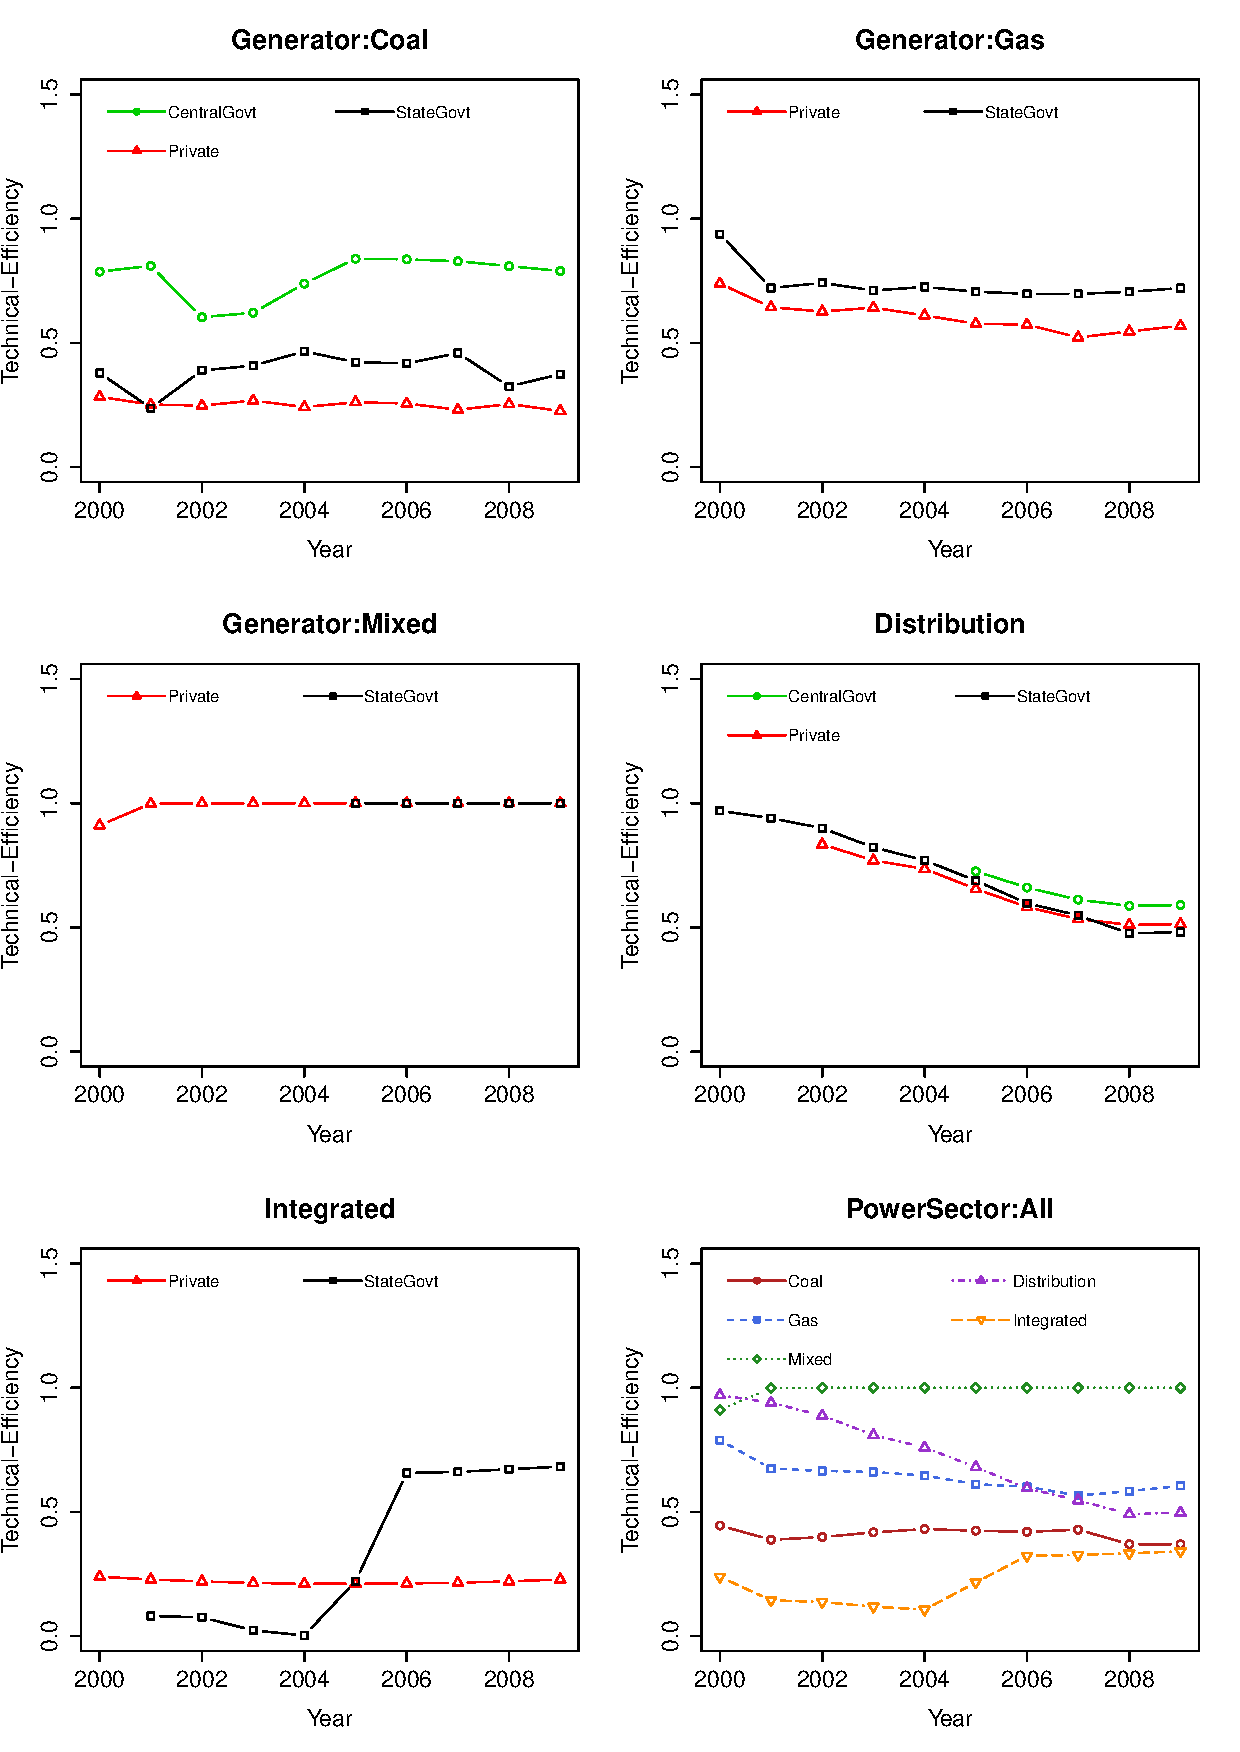
\includegraphics[width=1.00\textwidth]{chapter02/EffTimeTrend.pdf}	
\end{figure}

\begin{figure}[h]
	\centering
	\caption{Power Sector Technical Efficiency Distribution}
	\label{fig:EffDistr}
		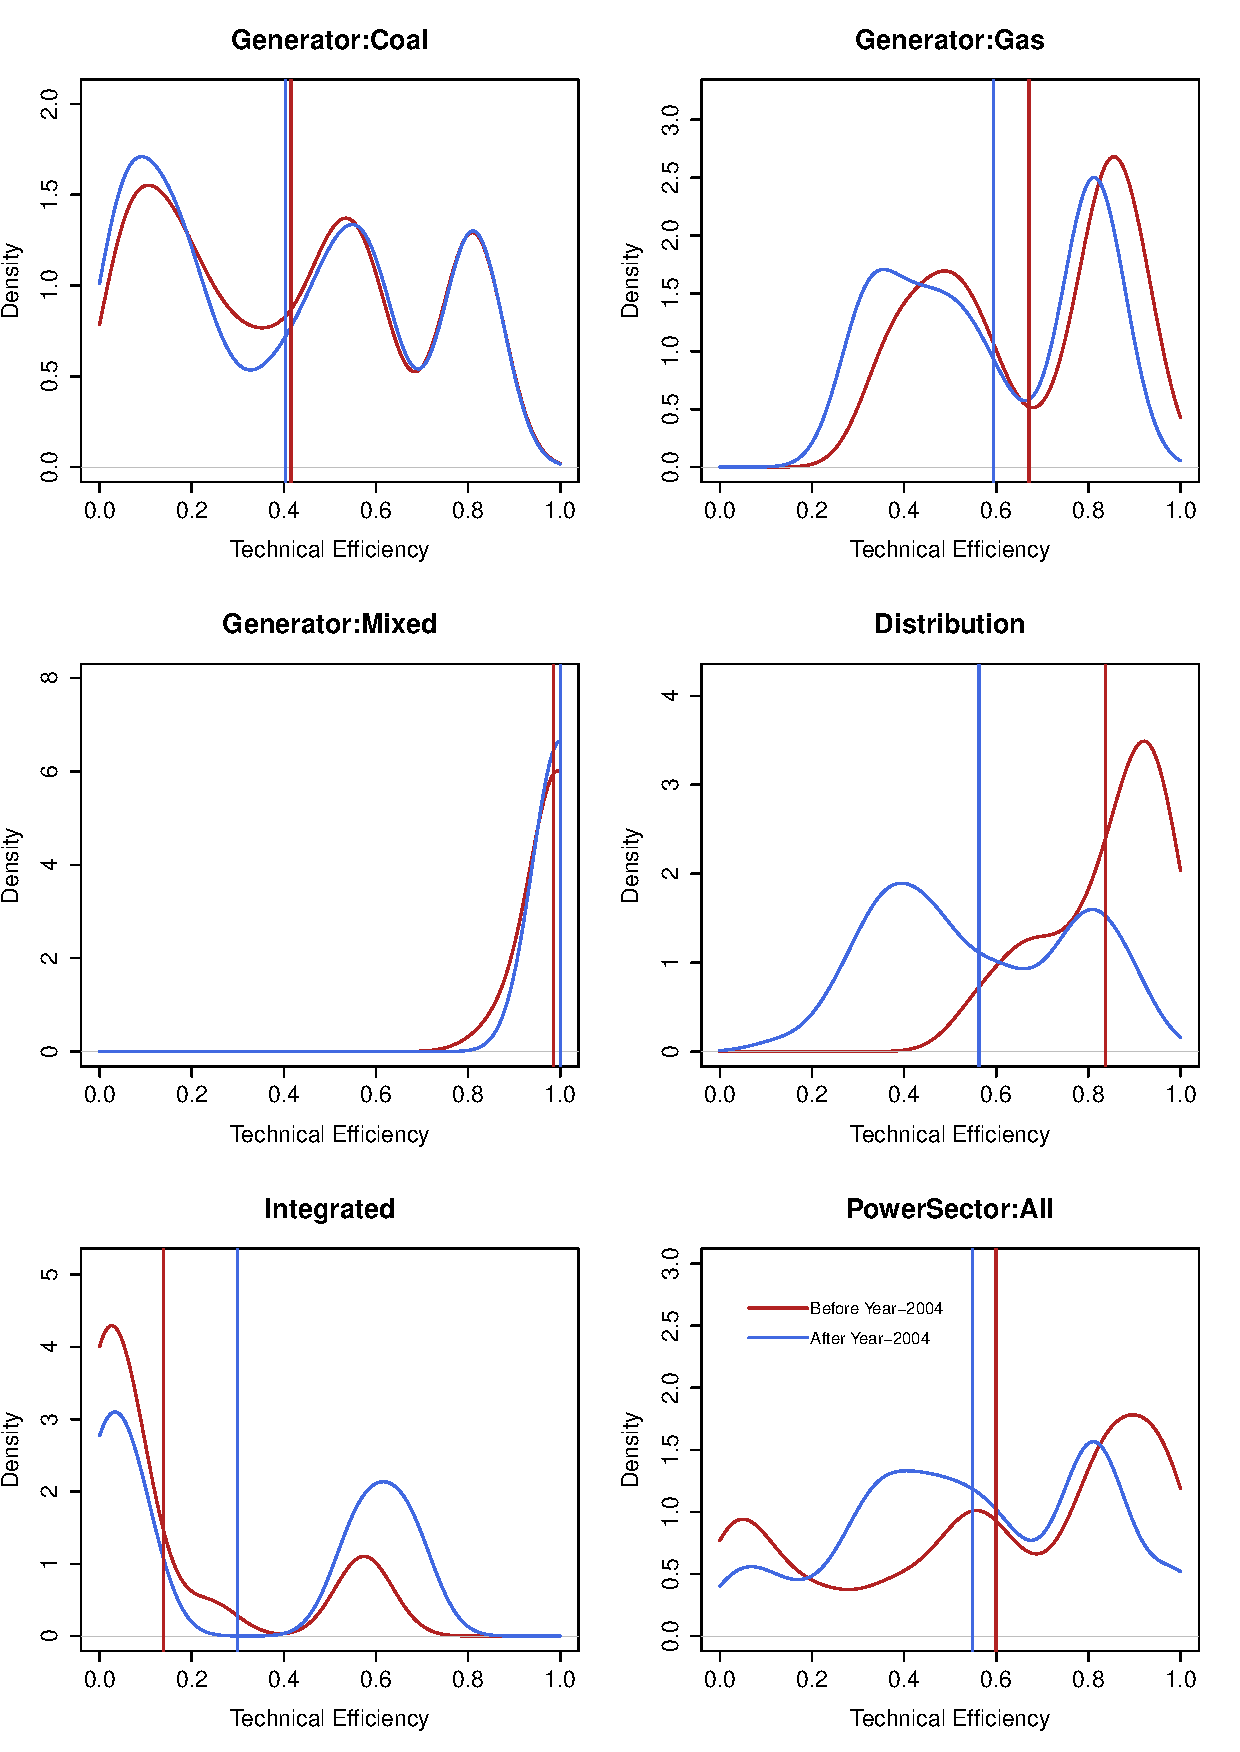
\includegraphics[width=1.00\textwidth]{chapter02/EffDistr.pdf}	
\end{figure}

\begin{figure}[h]
\centering
\caption{TFP Change in Power Sector}
	\label{fig:TFPChange}
	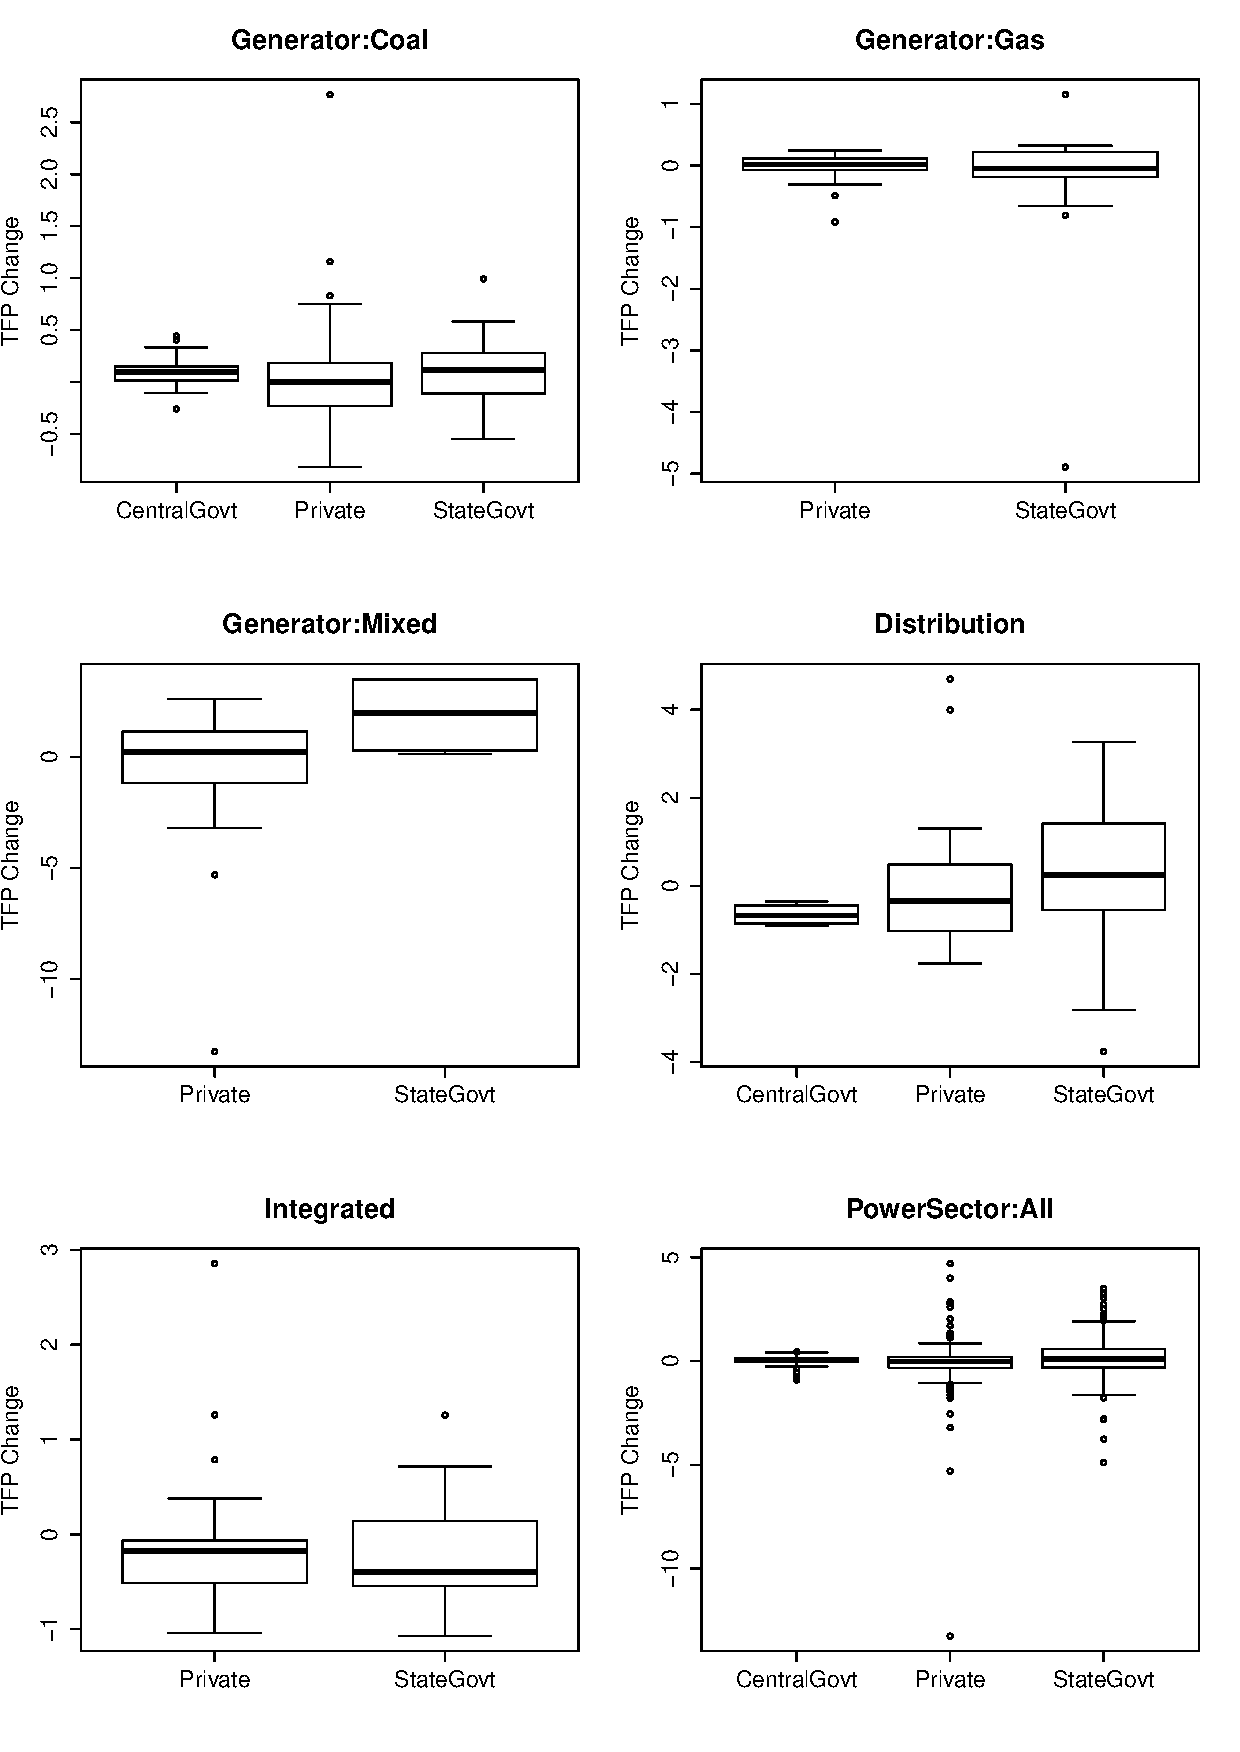
\includegraphics[width=1.00\textwidth]{chapter02/TFPChange.pdf}	
\end{figure}

\begin{figure}[h]
	\centering
	\caption{Technical Change in Power Sector}
	\label{fig:TechChange}
		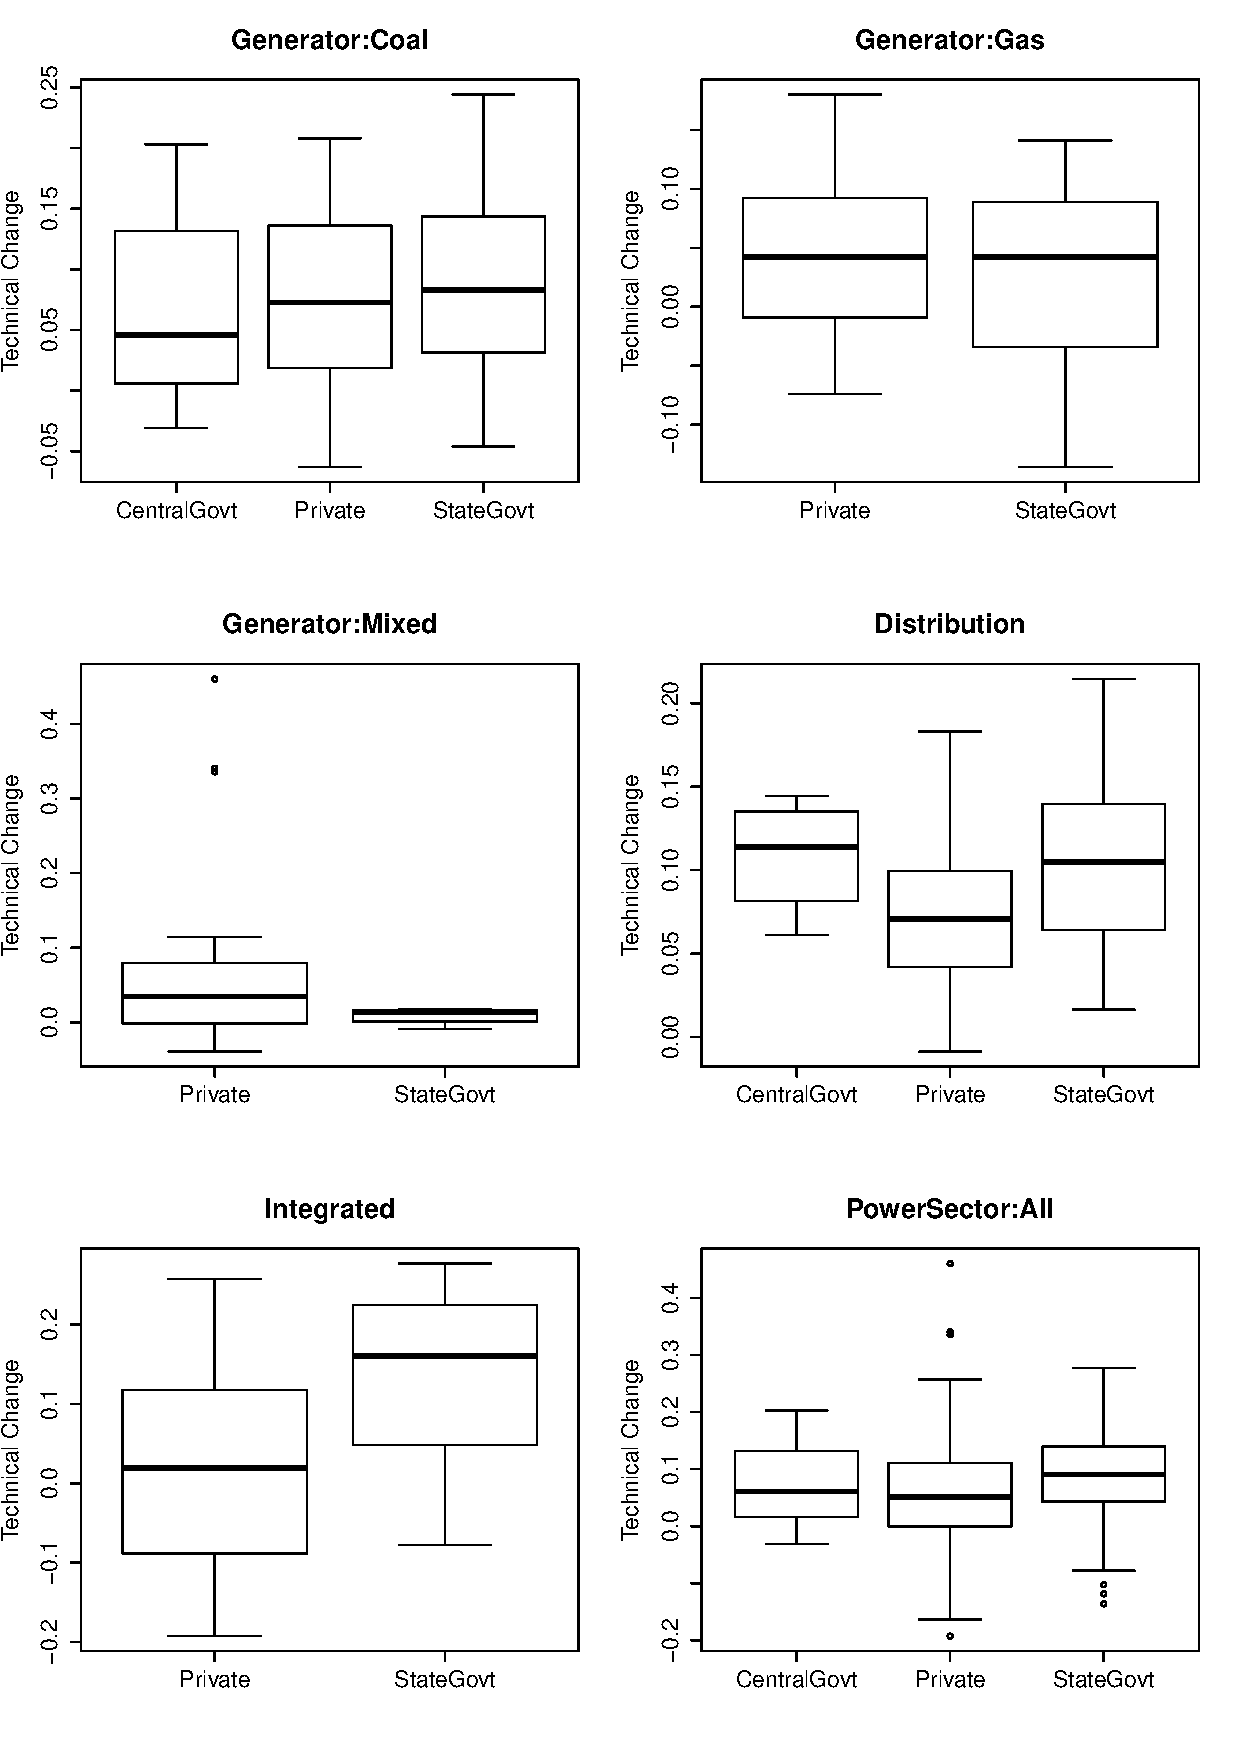
\includegraphics[width=1.00\textwidth]{chapter02/TechChange.pdf}	
\end{figure}

\begin{figure}[h]
\centering
\caption{Efficiency Change in Power Sector}
	\label{fig:EffChange}
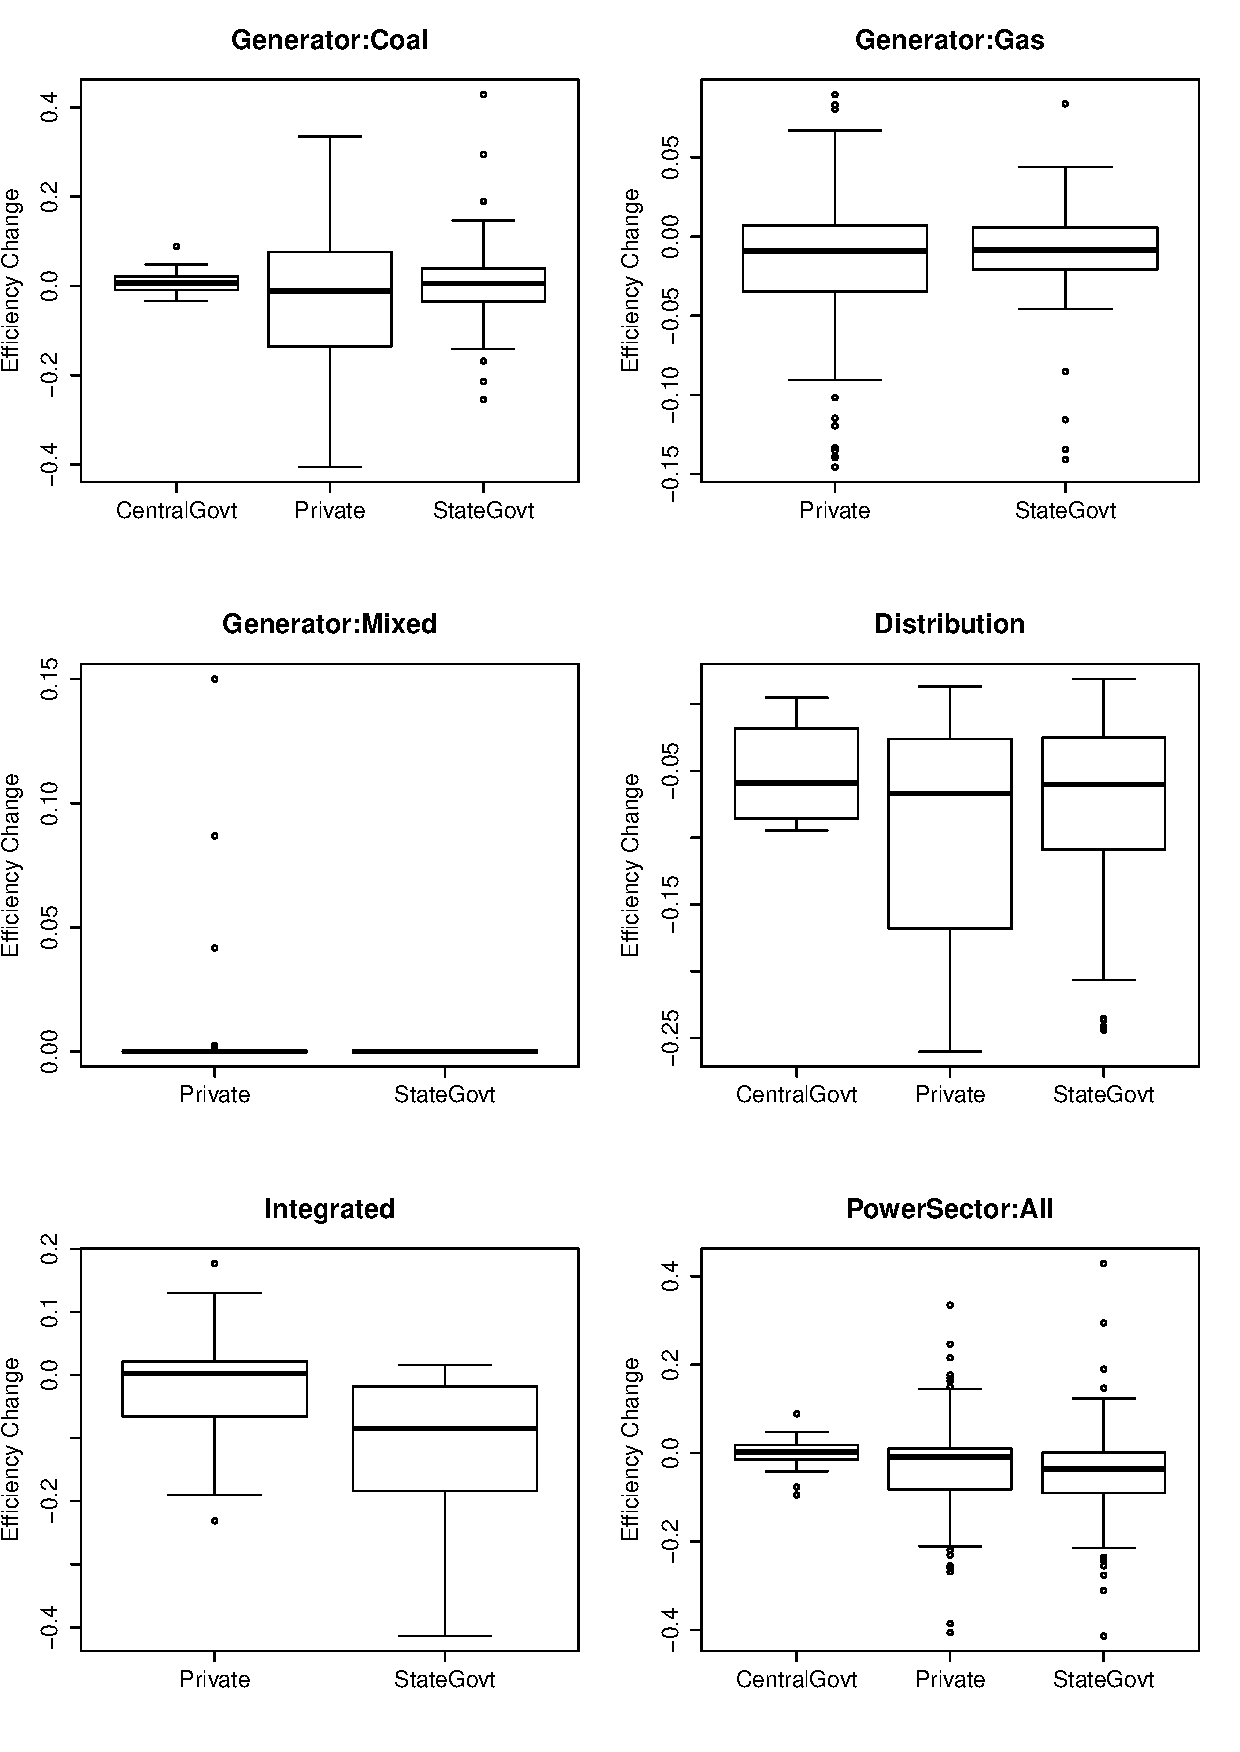
\includegraphics[width=1.00\textwidth]{chapter02/EffChange.pdf}\\		
\end{figure}

\begin{figure}[h]
\centering
\caption{Scale Effect on TFP Change in Power Sector}
	\label{fig:ScaleChange}
	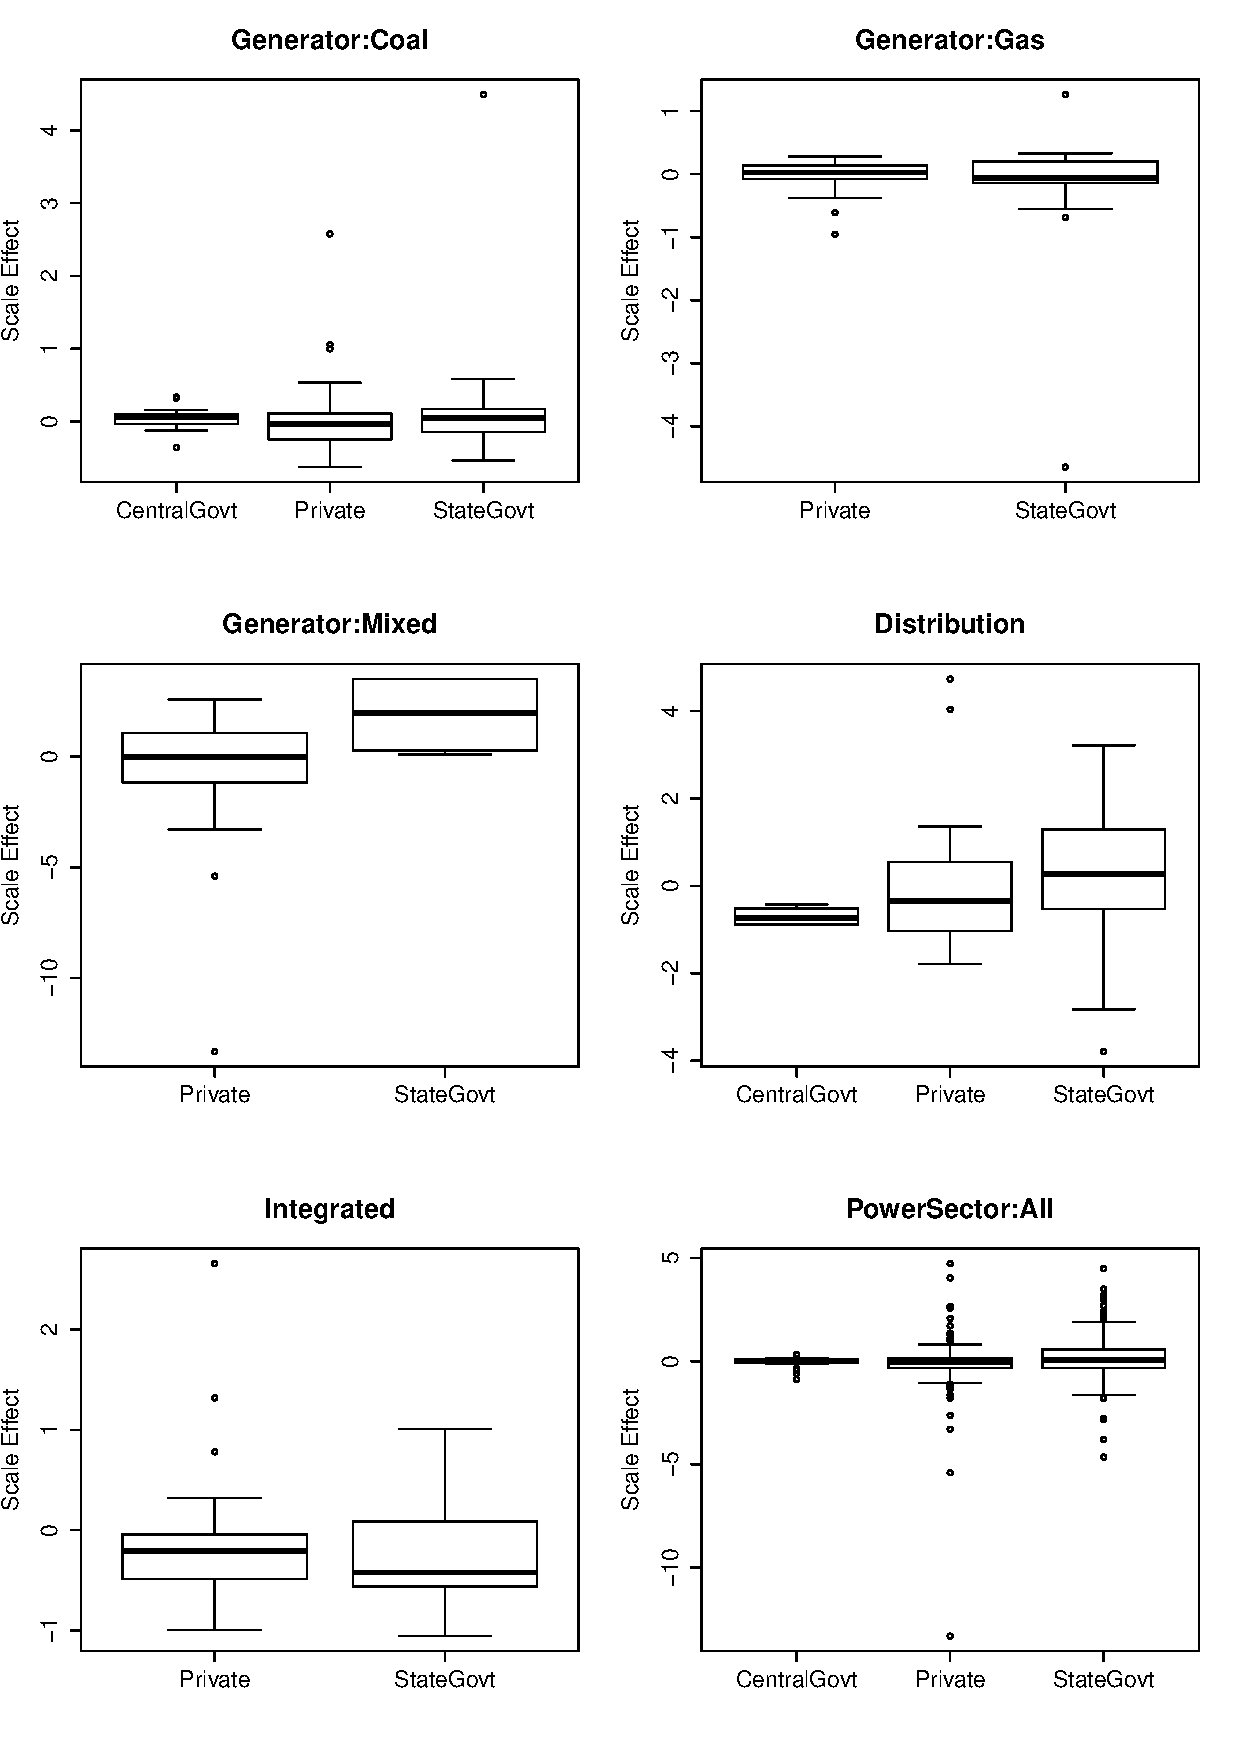
\includegraphics[width=1.00\textwidth]{chapter02/ScaleChange.pdf}	
\end{figure}

\begin{figure}[h]
\centering
\caption{Price Effect on TFP Change in Power Sector}
	\label{fig:PriceChange}
	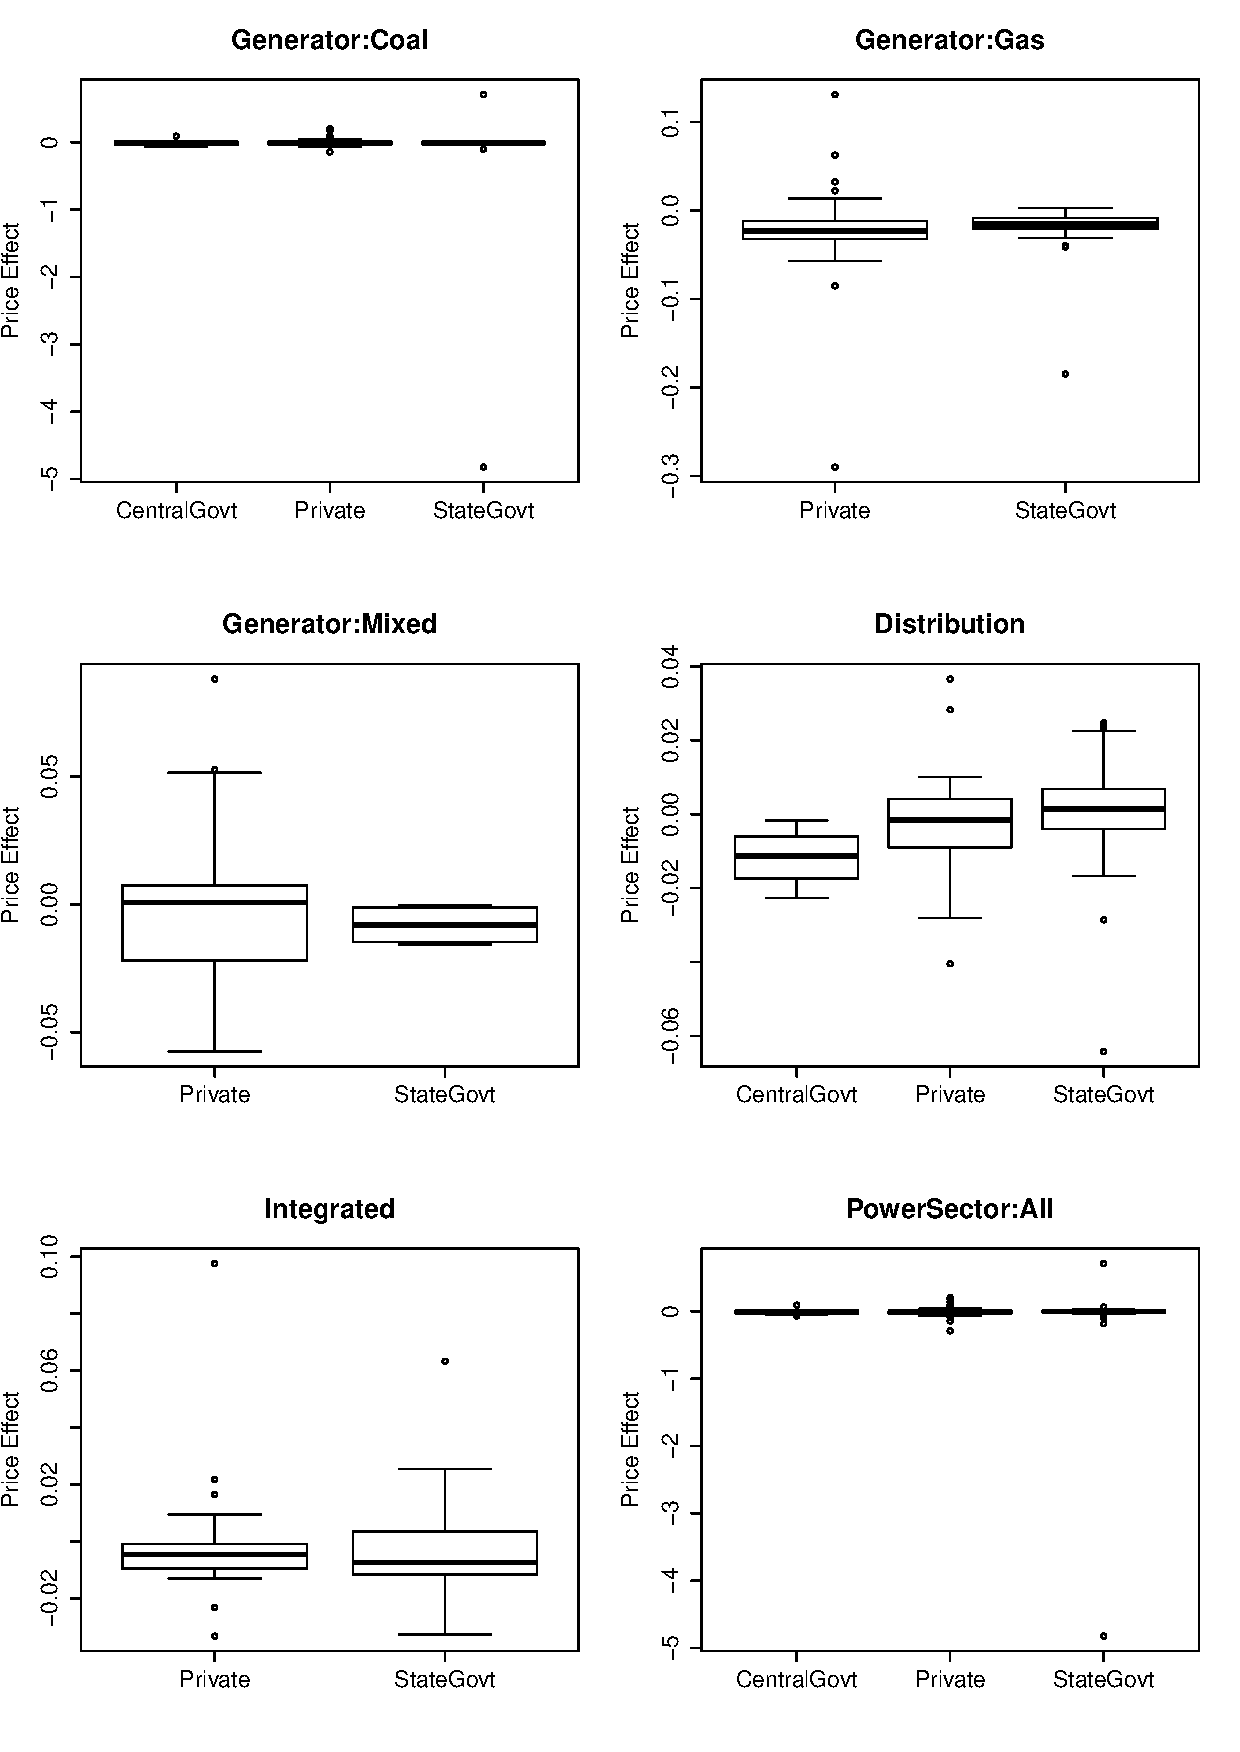
\includegraphics[width=1.00\textwidth]{chapter02/PriceChange.pdf}	
\end{figure}






\bibliographystyle{apalike} 
\onehalfspacing
%\singlespacing
\bibliography{chap02refs}
%\doublespacing

